\documentclass[12pt]{beamer}
\usepackage{amsmath}
\usepackage{booktabs}
\usepackage{pgf}
%\usepackage[UTF8,noindent]{ctexcap}
\usepackage{mathptmx}
\usepackage{helvet}
\usepackage[T1]{fontenc}
\usepackage{lmodern}
\usebeamerfont{frametitle}
\usefonttheme{professionalfonts}
\usepackage{graphicx}
\usepackage{physics}
%\usepackage{multimedia}
\usepackage{media9}

%\usetheme{AnnArbor}
\usetheme{CambridgeUS}

\title[1d MHD code]{One-dimensional MHD code tests}
\author[Xuyao Hu]{Xuyao Hu}
\institute[NYU]{Department of Physics, New York University}
\date{\today}

\AtBeginSection[]{
	\begin{frame}
	\tableofcontents[currentsection]
\end{frame}
}
\AtBeginSubsection[]{
	\begin{frame}
	\tableofcontents[currentsubsection]
\end{frame}
}

\begin{document}
\maketitle

\begin{frame}{Contents}	
	\tableofcontents
\end{frame}

%Section 1: Introduction
\section{Introduction -- MHD system}
\begin{frame}{Introduction -- MHD system}
Magnetohydrodynamics (MHD) is extremely important in various fields such as 
Astrophysics, Geophysics and Plasma Physics.\\ 
An ideal MHD system is governed by hydrodynamics equations and Maxwell's equations,
which can be written in a conservative form as
 \begin{align}
 	&\pdv{\rho}{t}+\div (\rho \vb*{v})=0 \ , \\
	&\pdv{\rho \vb*{v}}{t} +\div (\rho \vb*{v}\vb*{v}-\vb*{B}\vb*{B}+\vb*{P}_T)=0 \ , \\
	&\pdv{E}{t} + \div [(E+P_T)\vb*{v}-\vb*{B}(\vb*{B}\vdot\vb*{v})]=0 \ , \\
	&\pdv{\vb*{B}}{t}-\curl (\vb*{v} \cross \vb*{B})=0 \ ,
 \end{align}
 where $P_T=P+\frac{1}{2}B^2$.

\end{frame}

\begin{frame}{Introduction -- 1D MHD problem}
``One-dimensional'' $\Longrightarrow$ All physical quantities depends only on \textbf{one} 
position variable (say, $x$ in 3D Cartesian coordinates) and time $t$.
\begin{align}
	\pdv{\vb*{U}}{t}+\pdv{\vb*{F}}{x}=0 \ ,
\end{align}
with
\begin{align}
	\vb*{U}=\begin{pmatrix}
	\rho \\
	\rho v_x \\
	\rho v_y \\
	\rho v_z \\
	E \\
	B_y \\
	B_z
	\end{pmatrix} \ , 
	\qquad 
	\vb*{F}=\begin{pmatrix}
	\rho v_x \\
	\rho v_x^2 + P_T -B_x^2 \\
	\rho v_x v_y - B_x B_y \\
	\rho v_x v_z - B_x B_z \\
	(E+P_T)v_x - (\vb*{B}\vdot\vb*{v}) B_x \\
	B_y v_x - B_x v_y \\
	B_z v_x - B_x v_z
	\end{pmatrix} \ ,
\end{align}
and $B_x = \text{constant}$.
\end{frame}


%Section 2: Algorithm
\section{Algorithm}
\begin{frame}{Algorithm -- Piecewise Linear Method (PLM)}
Use PLM to reconstruct the ``left'' and ``right'' states at each cell interface
\begin{align}
	Q^L_{i+1/2} &= Q_i + 0.5\ \text{minmod}(\theta(Q_i-Q_{i-1}),0.5(Q_{i+1}-Q_{i-1}), \notag \\ &\theta(Q_{i+1}-Q_i)) \ , 
	\label{eq: PLM_eq1}\\
	Q^R_{i+1/2}&= Q_{i+1} - 0.5\ \text{minmod}(\theta(Q_{i+1}-Q_{i}),0.5(Q_{i+2}-Q_{i}), \notag \\ &\theta(Q_{i+2}-Q_{i+1})) \ ,
	\label{eq: PLM_eq2}
\end{align}
where $\theta = 1.1$, $Q$ denotes $\rho,\ v_x,\ v_y,\ v_z,\ P,\ B_x,\ B_y,\ B_z$.
\end{frame}

\begin{frame}{Algorithm -- HLL vs. HLLD}
\begin{itemize}
	\item \textbf{HLL} -- determine the flow through each interface using \textbf{one} 
	intermediate state\\
	\only<1>{\begin{align}
		\vb*{F}_{\text{HLL}} = \begin{cases}
			\vb*{F}_{\text{L}} & \text{if } S_L>0 \ ,  \\
			\vb*{F}^* & \text{if } S_L \leq 0 \leq S_R \ , \\
			\vb*{F}_{\text{R}} & \text{if } S_R<0 \ .
		\end{cases}
	\end{align}}
\end{itemize}
\only<2>{
\begin{figure}[ht]
	\centering
	\begin{minipage}[c]{1\textwidth}
		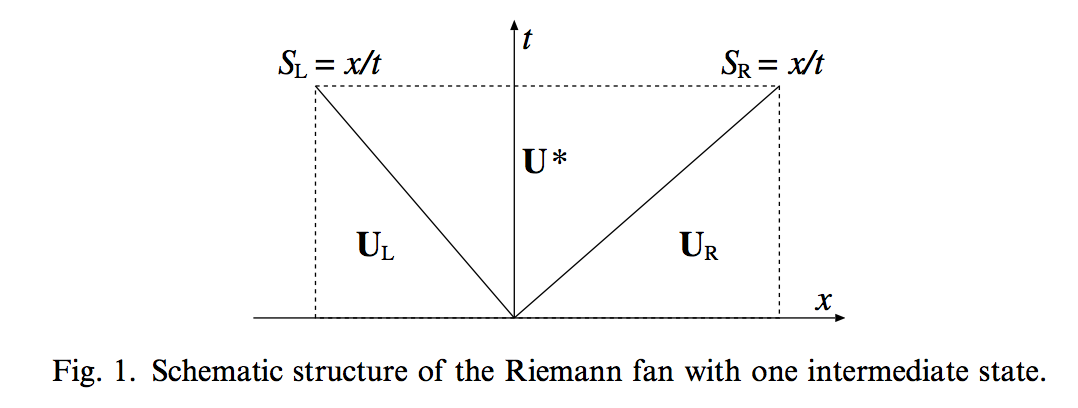
\includegraphics[width=1\textwidth]{HLL.png}
	\end{minipage}%
\end{figure}
}
\qquad \small{See Miyoshi \& Kusano (2005) for more details.}
\end{frame}

\begin{frame}{Algorithm -- HLL vs. HLLD}
\begin{itemize}
	\item \textbf{HLLD} -- determine the flow through each interface using \textbf{four}
	 intermediate state
	\\
	\only<1>{
	\begin{align}
		\vb*{F}_{\text{HLLD}} = \begin{cases}
			\vb*{F}_{\text{L}} & \text{if } S_L>0 \ ,  \\
			\vb*{F}^*_{\text{L}} & \text{if } S_L \leq 0 \leq S^*_L \ , \\
			\vb*{F}^{**}_{\text{L}} & \text{if } S^*_L \leq 0 \leq S_M \ , \\
			\vb*{F}^{**}_{\text{R}} & \text{if } S_M \leq 0 \leq S^*_R \ , \\
			\vb*{F}^{*}_{\text{R}} & \text{if } S^*_R \leq 0 \leq S_R \ , \\
			\vb*{F}_{\text{R}} & \text{if } S_R<0 \ .
		\end{cases}
	\end{align}
	}
\end{itemize}

\only<2>{
\begin{figure}[ht]
	\centering
	\begin{minipage}[c]{1\textwidth}
		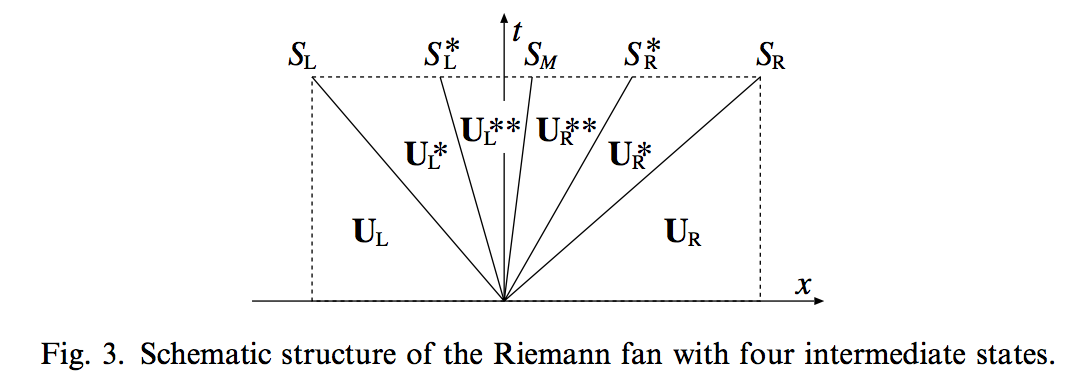
\includegraphics[width=1\textwidth]{HLLD.png}
	\end{minipage}%
\end{figure}}
\qquad \small{See Miyoshi \& Kusano (2005) for more details.}
\end{frame}

%Section 3: Numerical results
\section{Numerical results}
\begin{frame}{Dai \& Woodward shock tube}
\begin{figure}[ht]
	\centering
	\begin{minipage}[c]{1\textwidth}
		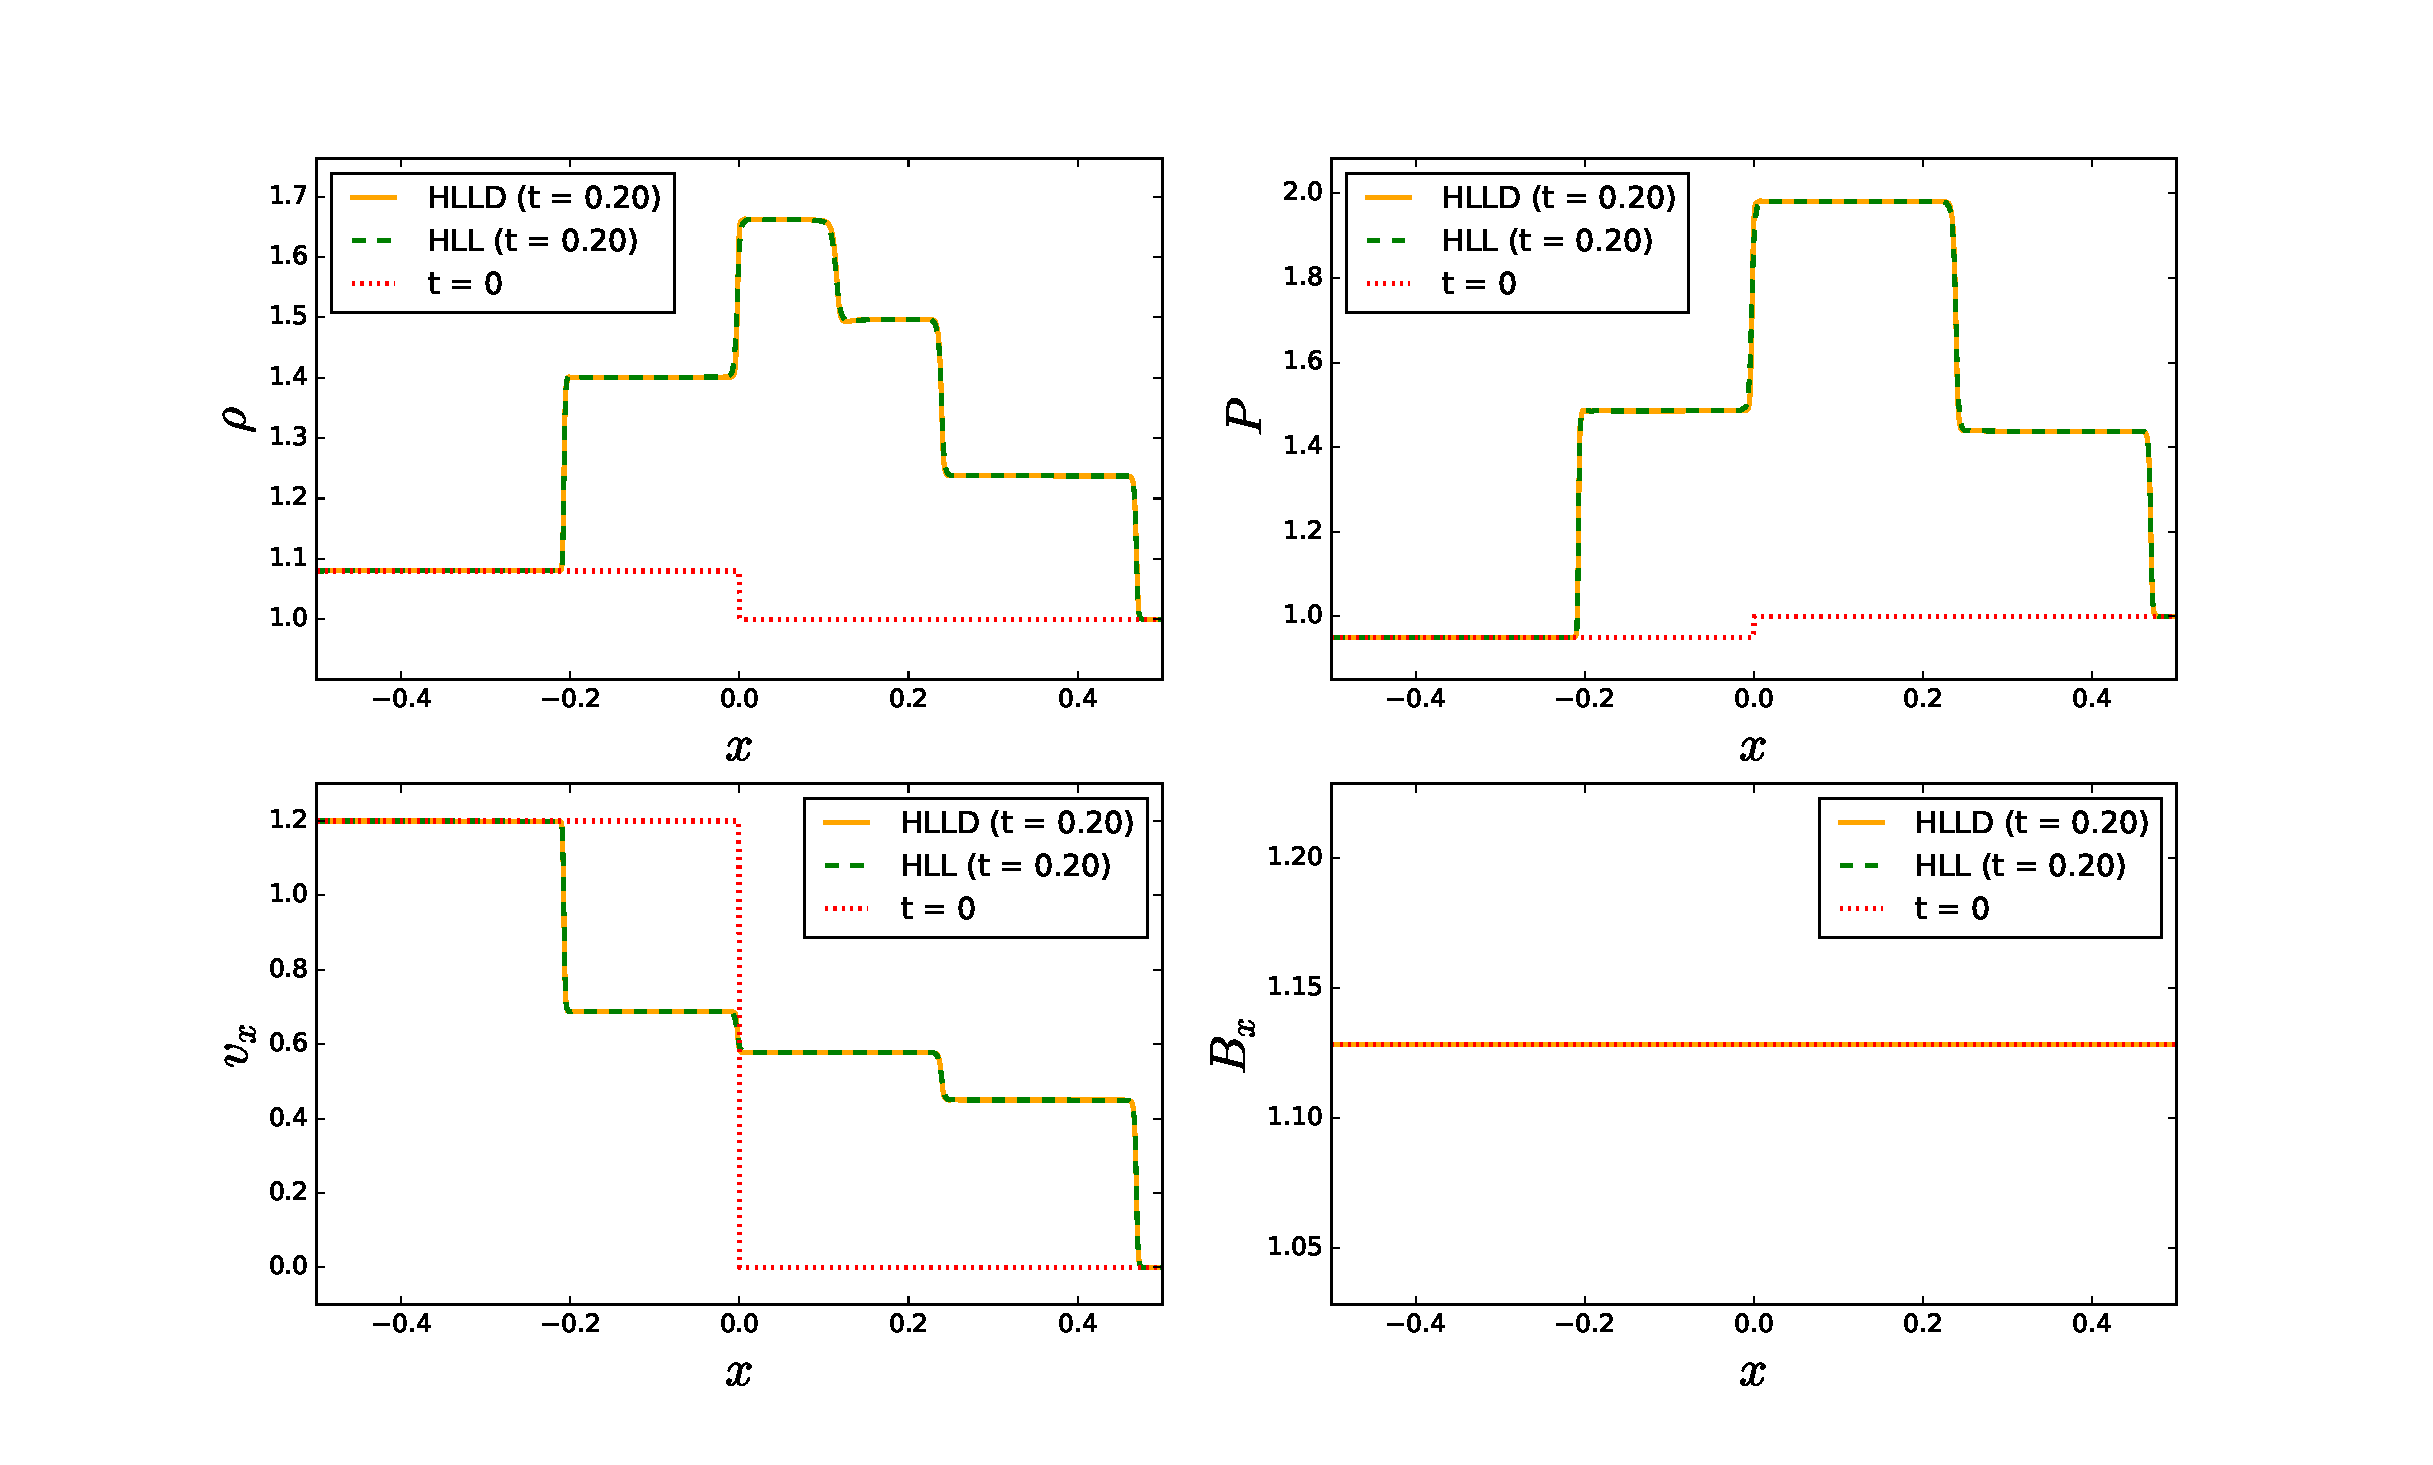
\includegraphics[width=1\textwidth]{DW1.eps}
	\end{minipage}%
\end{figure}
\end{frame}

\begin{frame}{Dai \& Woodward shock tube}
\only<1>{
\begin{figure}[ht]
	\centering
	\begin{minipage}[c]{1\textwidth}
		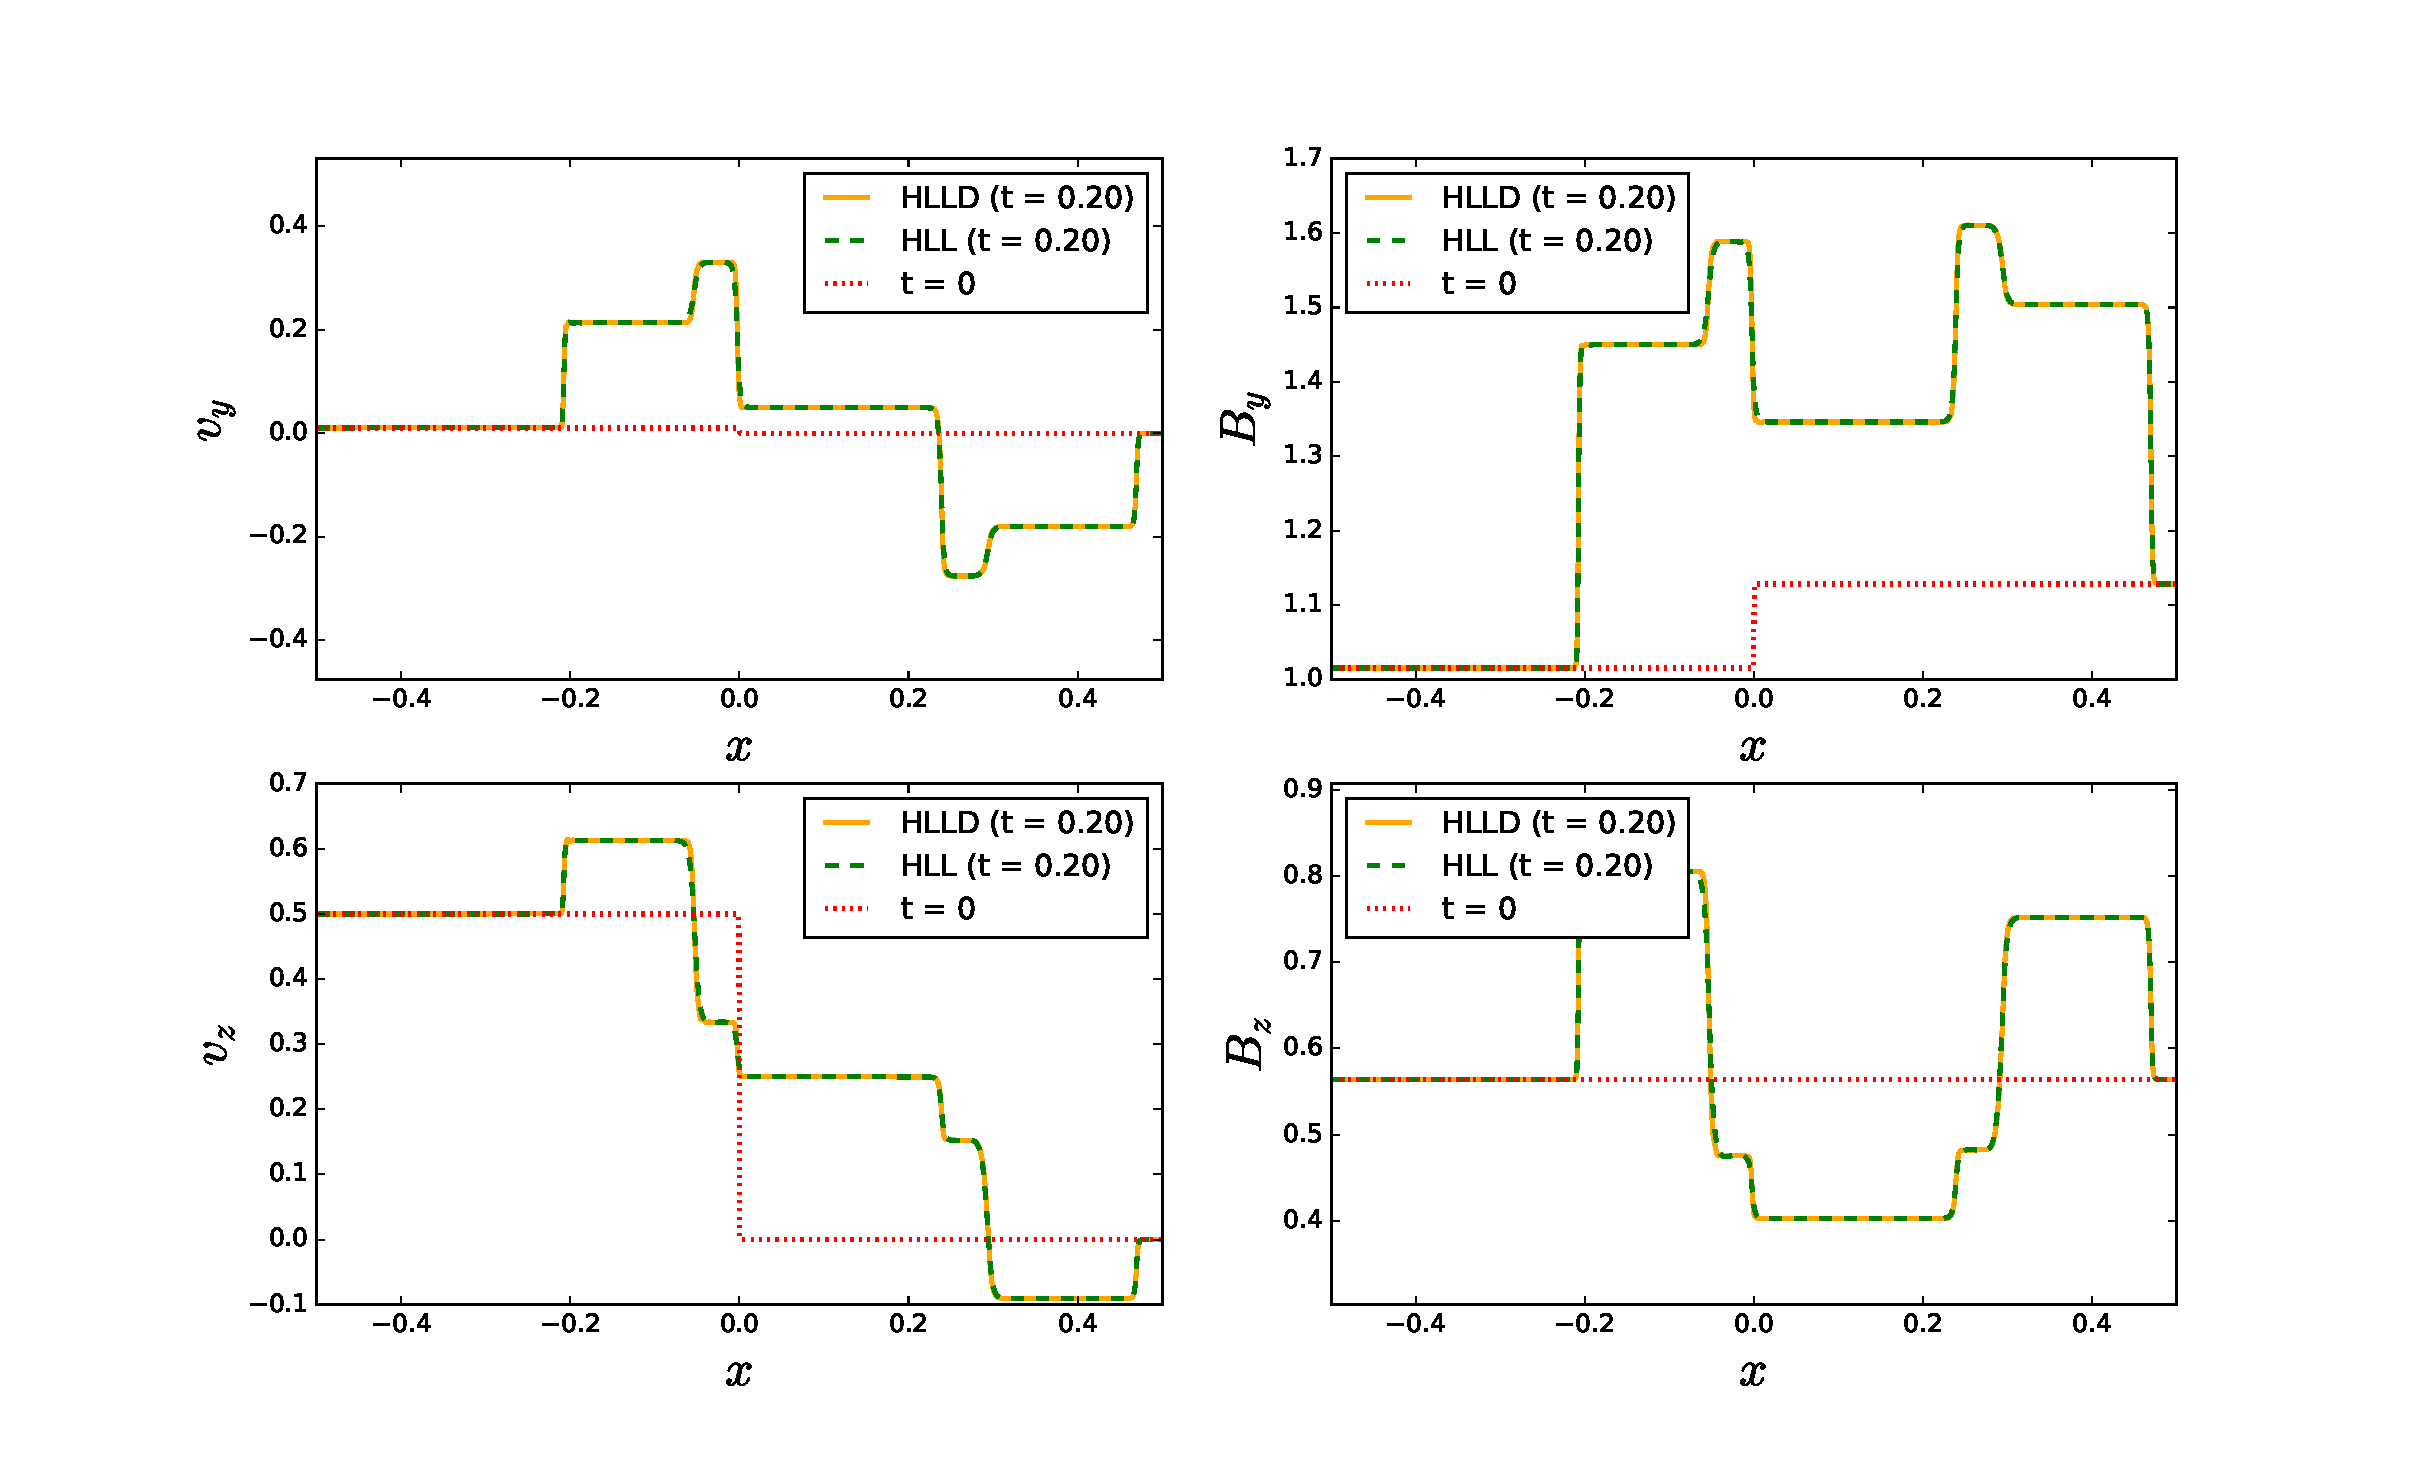
\includegraphics[width=1\textwidth]{DW2.eps}
	\end{minipage}%
\end{figure}
}
\only<2>{
\begin{figure}[ht]
	\centering
	\begin{minipage}[c]{1\textwidth}
		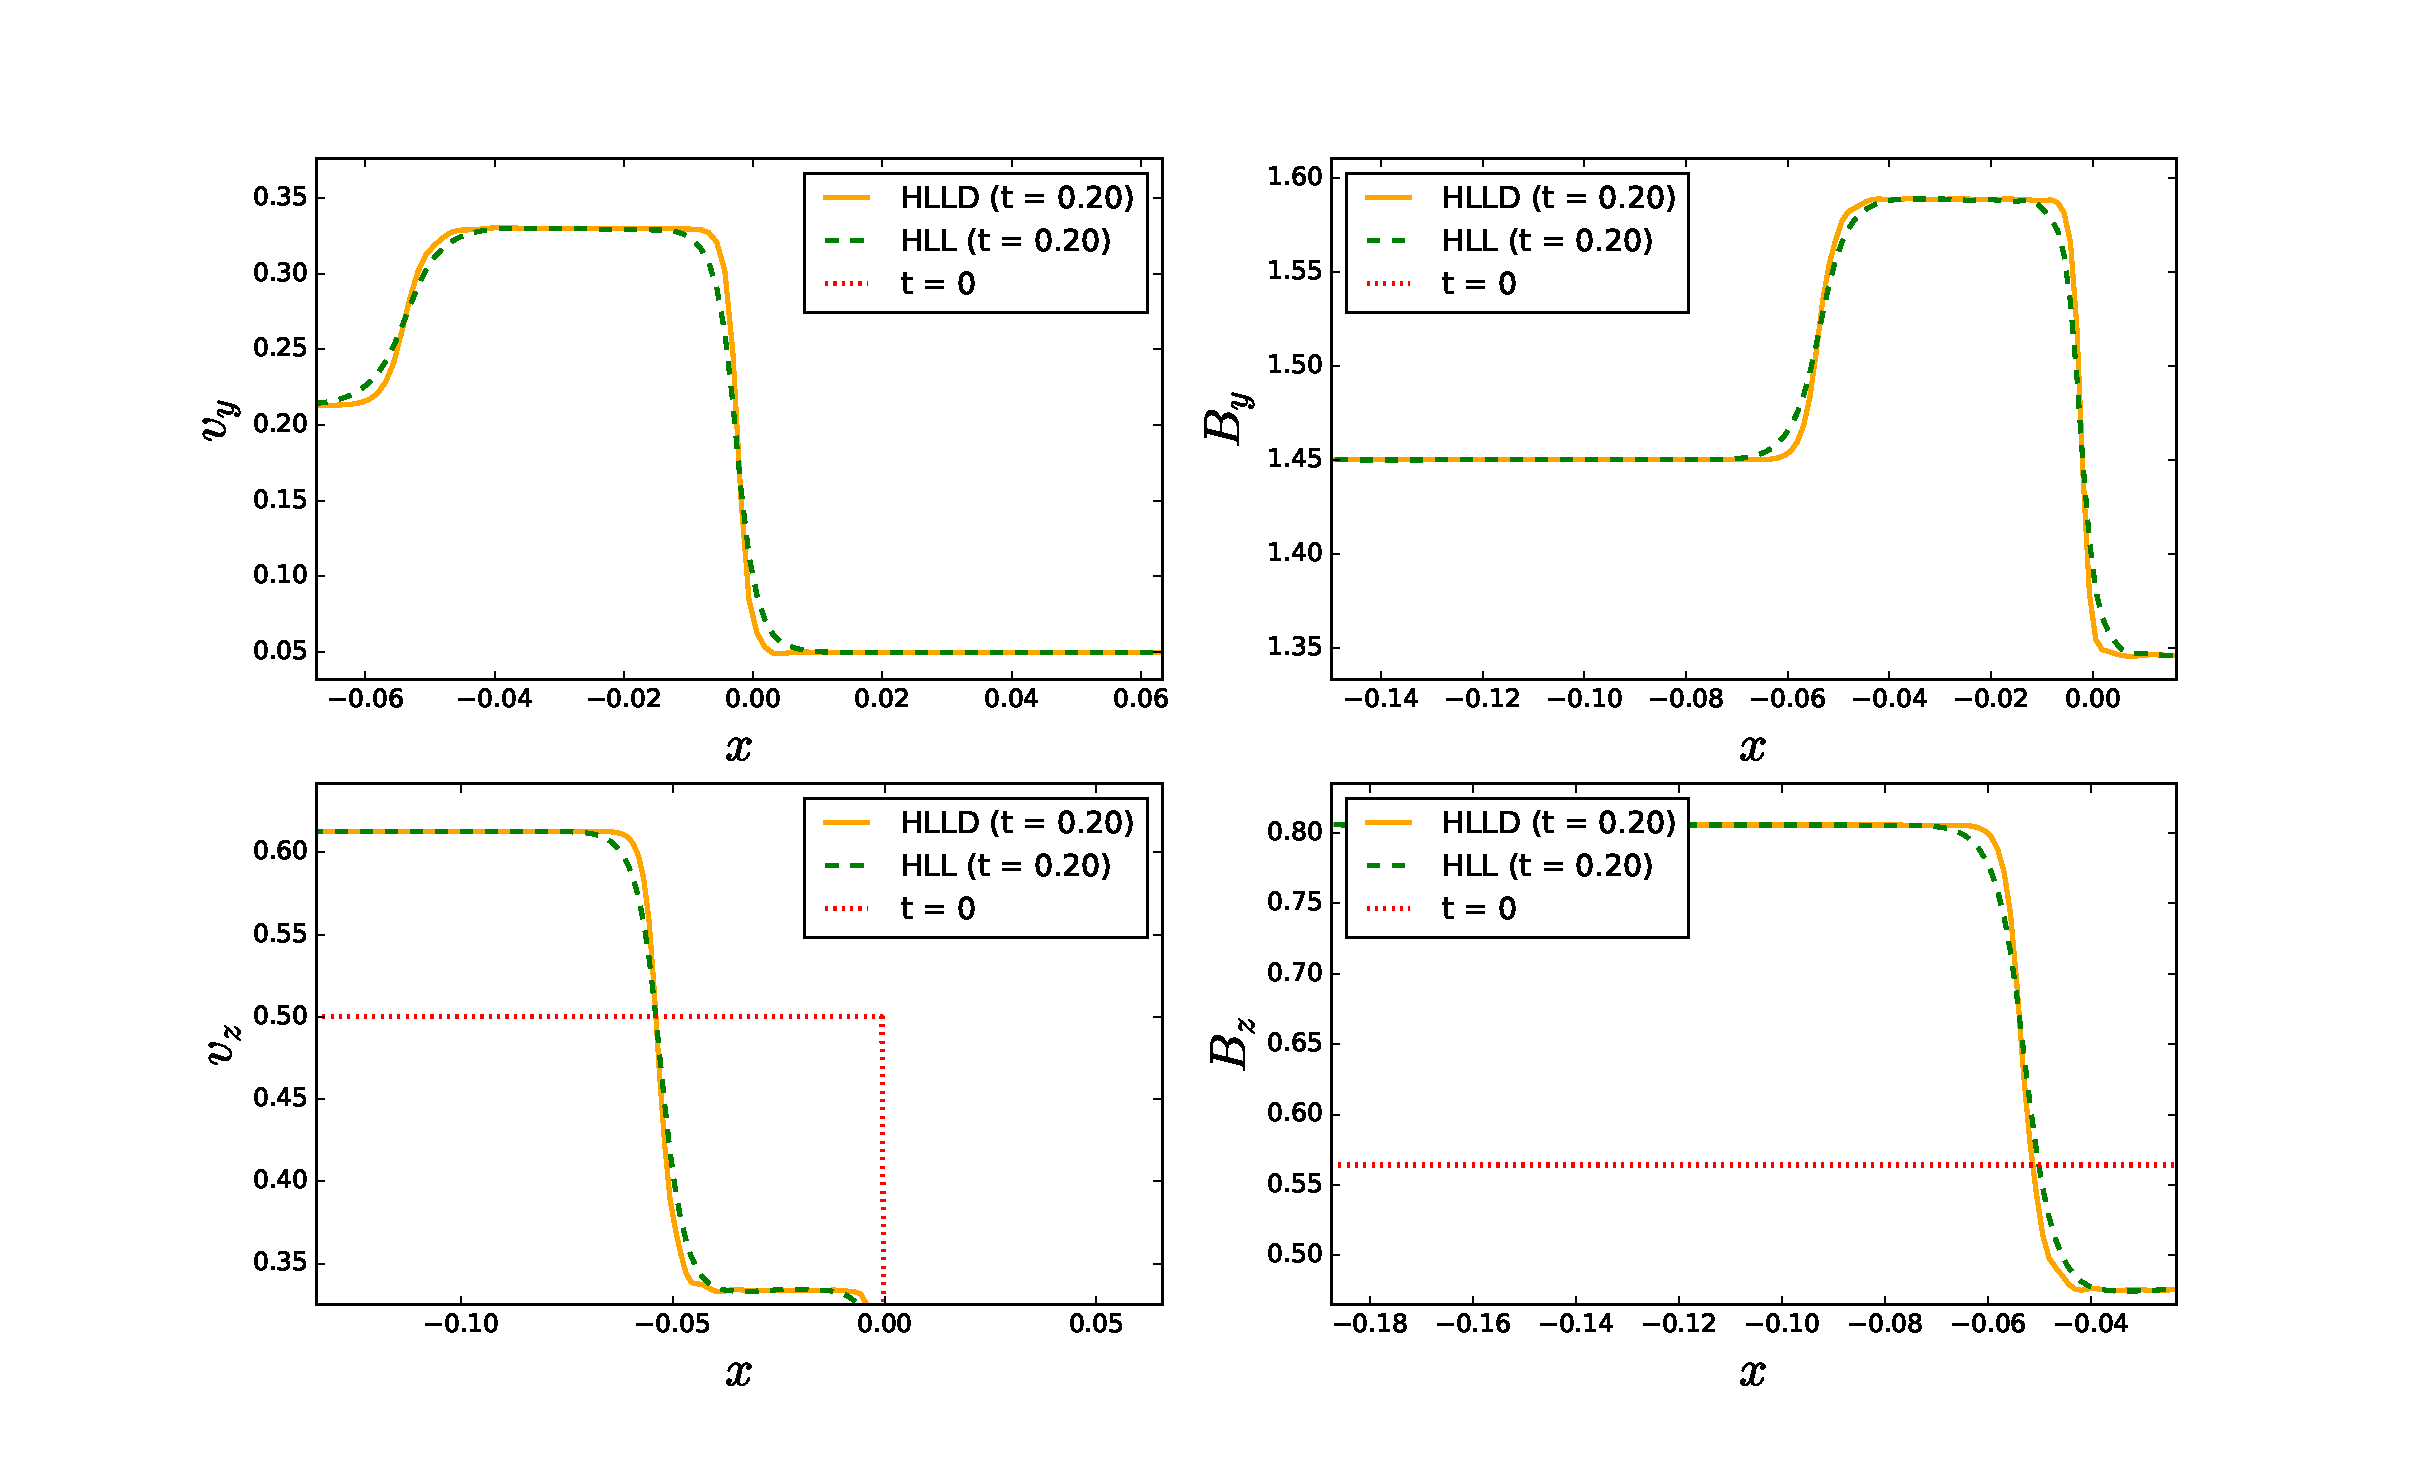
\includegraphics[width=1\textwidth]{DW2_zoomedin.eps}
	\end{minipage}%
\end{figure}
}
\end{frame}

\begin{frame}{Alfv\'en Wave}
\begin{figure}[ht]
	\centering
	\begin{minipage}[c]{1\textwidth}
		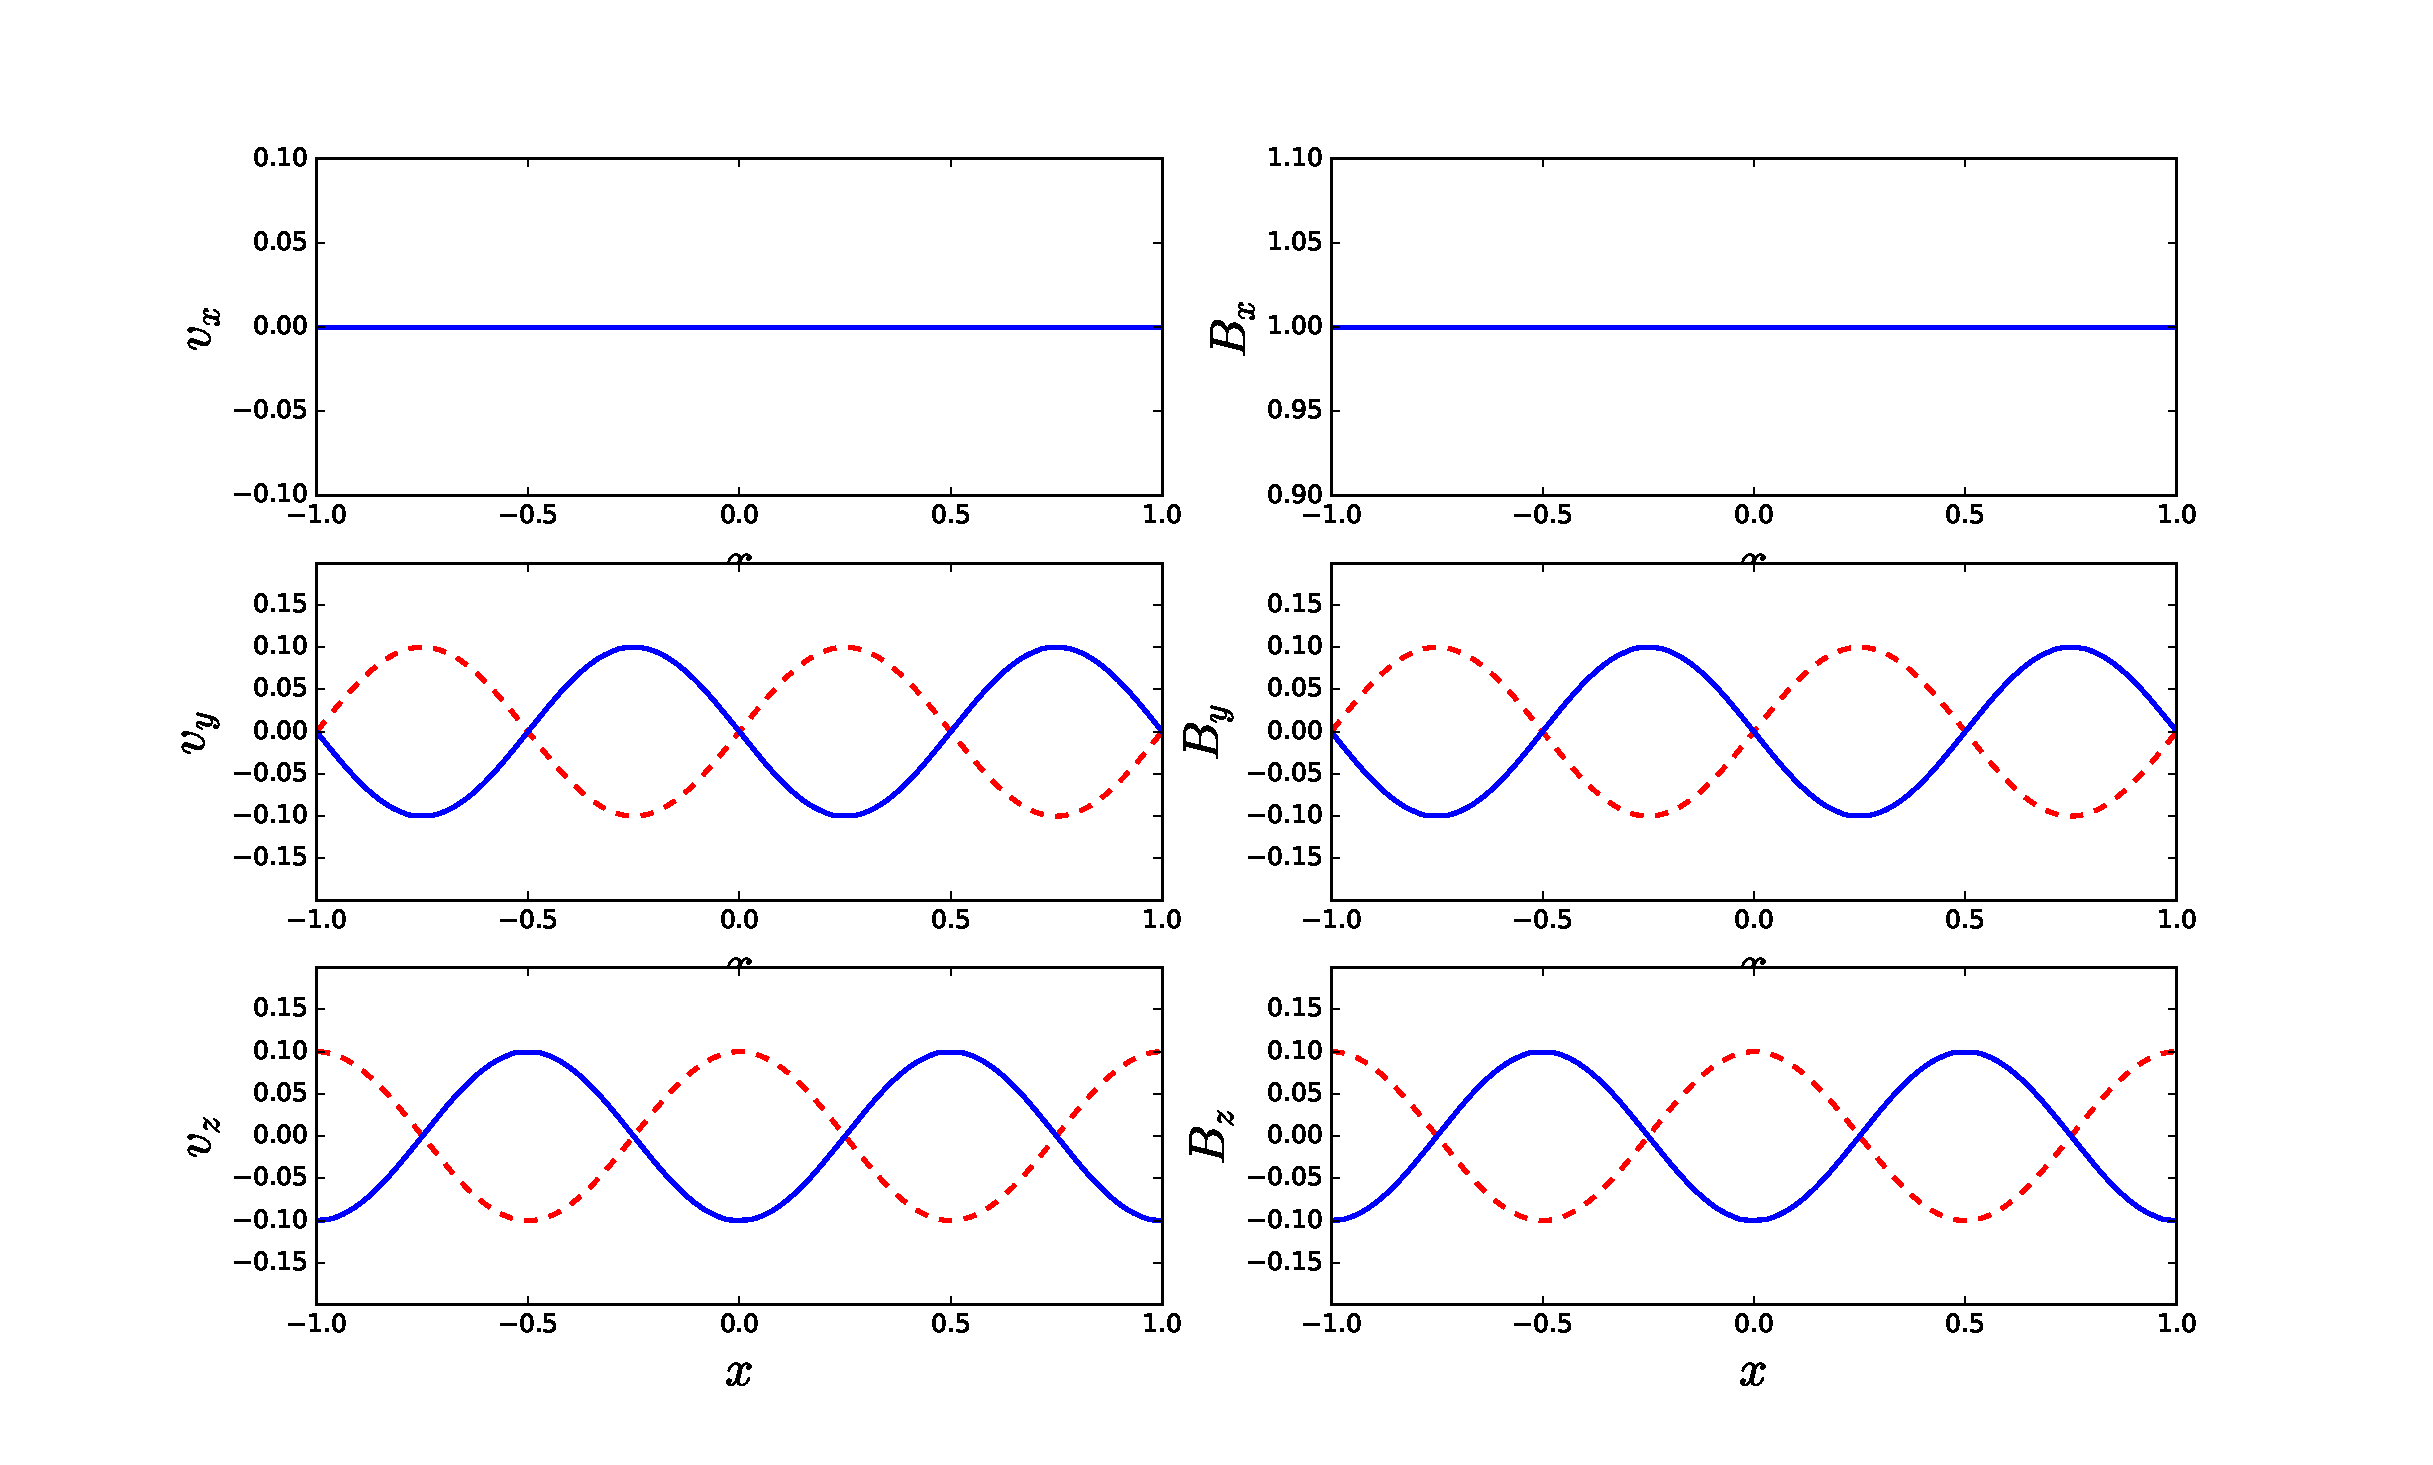
\includegraphics[width=1\textwidth]{AW.eps}
	\end{minipage}%
\end{figure}
\tiny{$t_{\text{final}} =2.5$. The density $\rho$ and the pressure $P$ basically remain constant.}
\end{frame}

\begin{frame}{Fast Switch-on (FS) shock test}
\only<1>{
\begin{figure}[ht]
	\centering
	\begin{minipage}[c]{1\textwidth}
		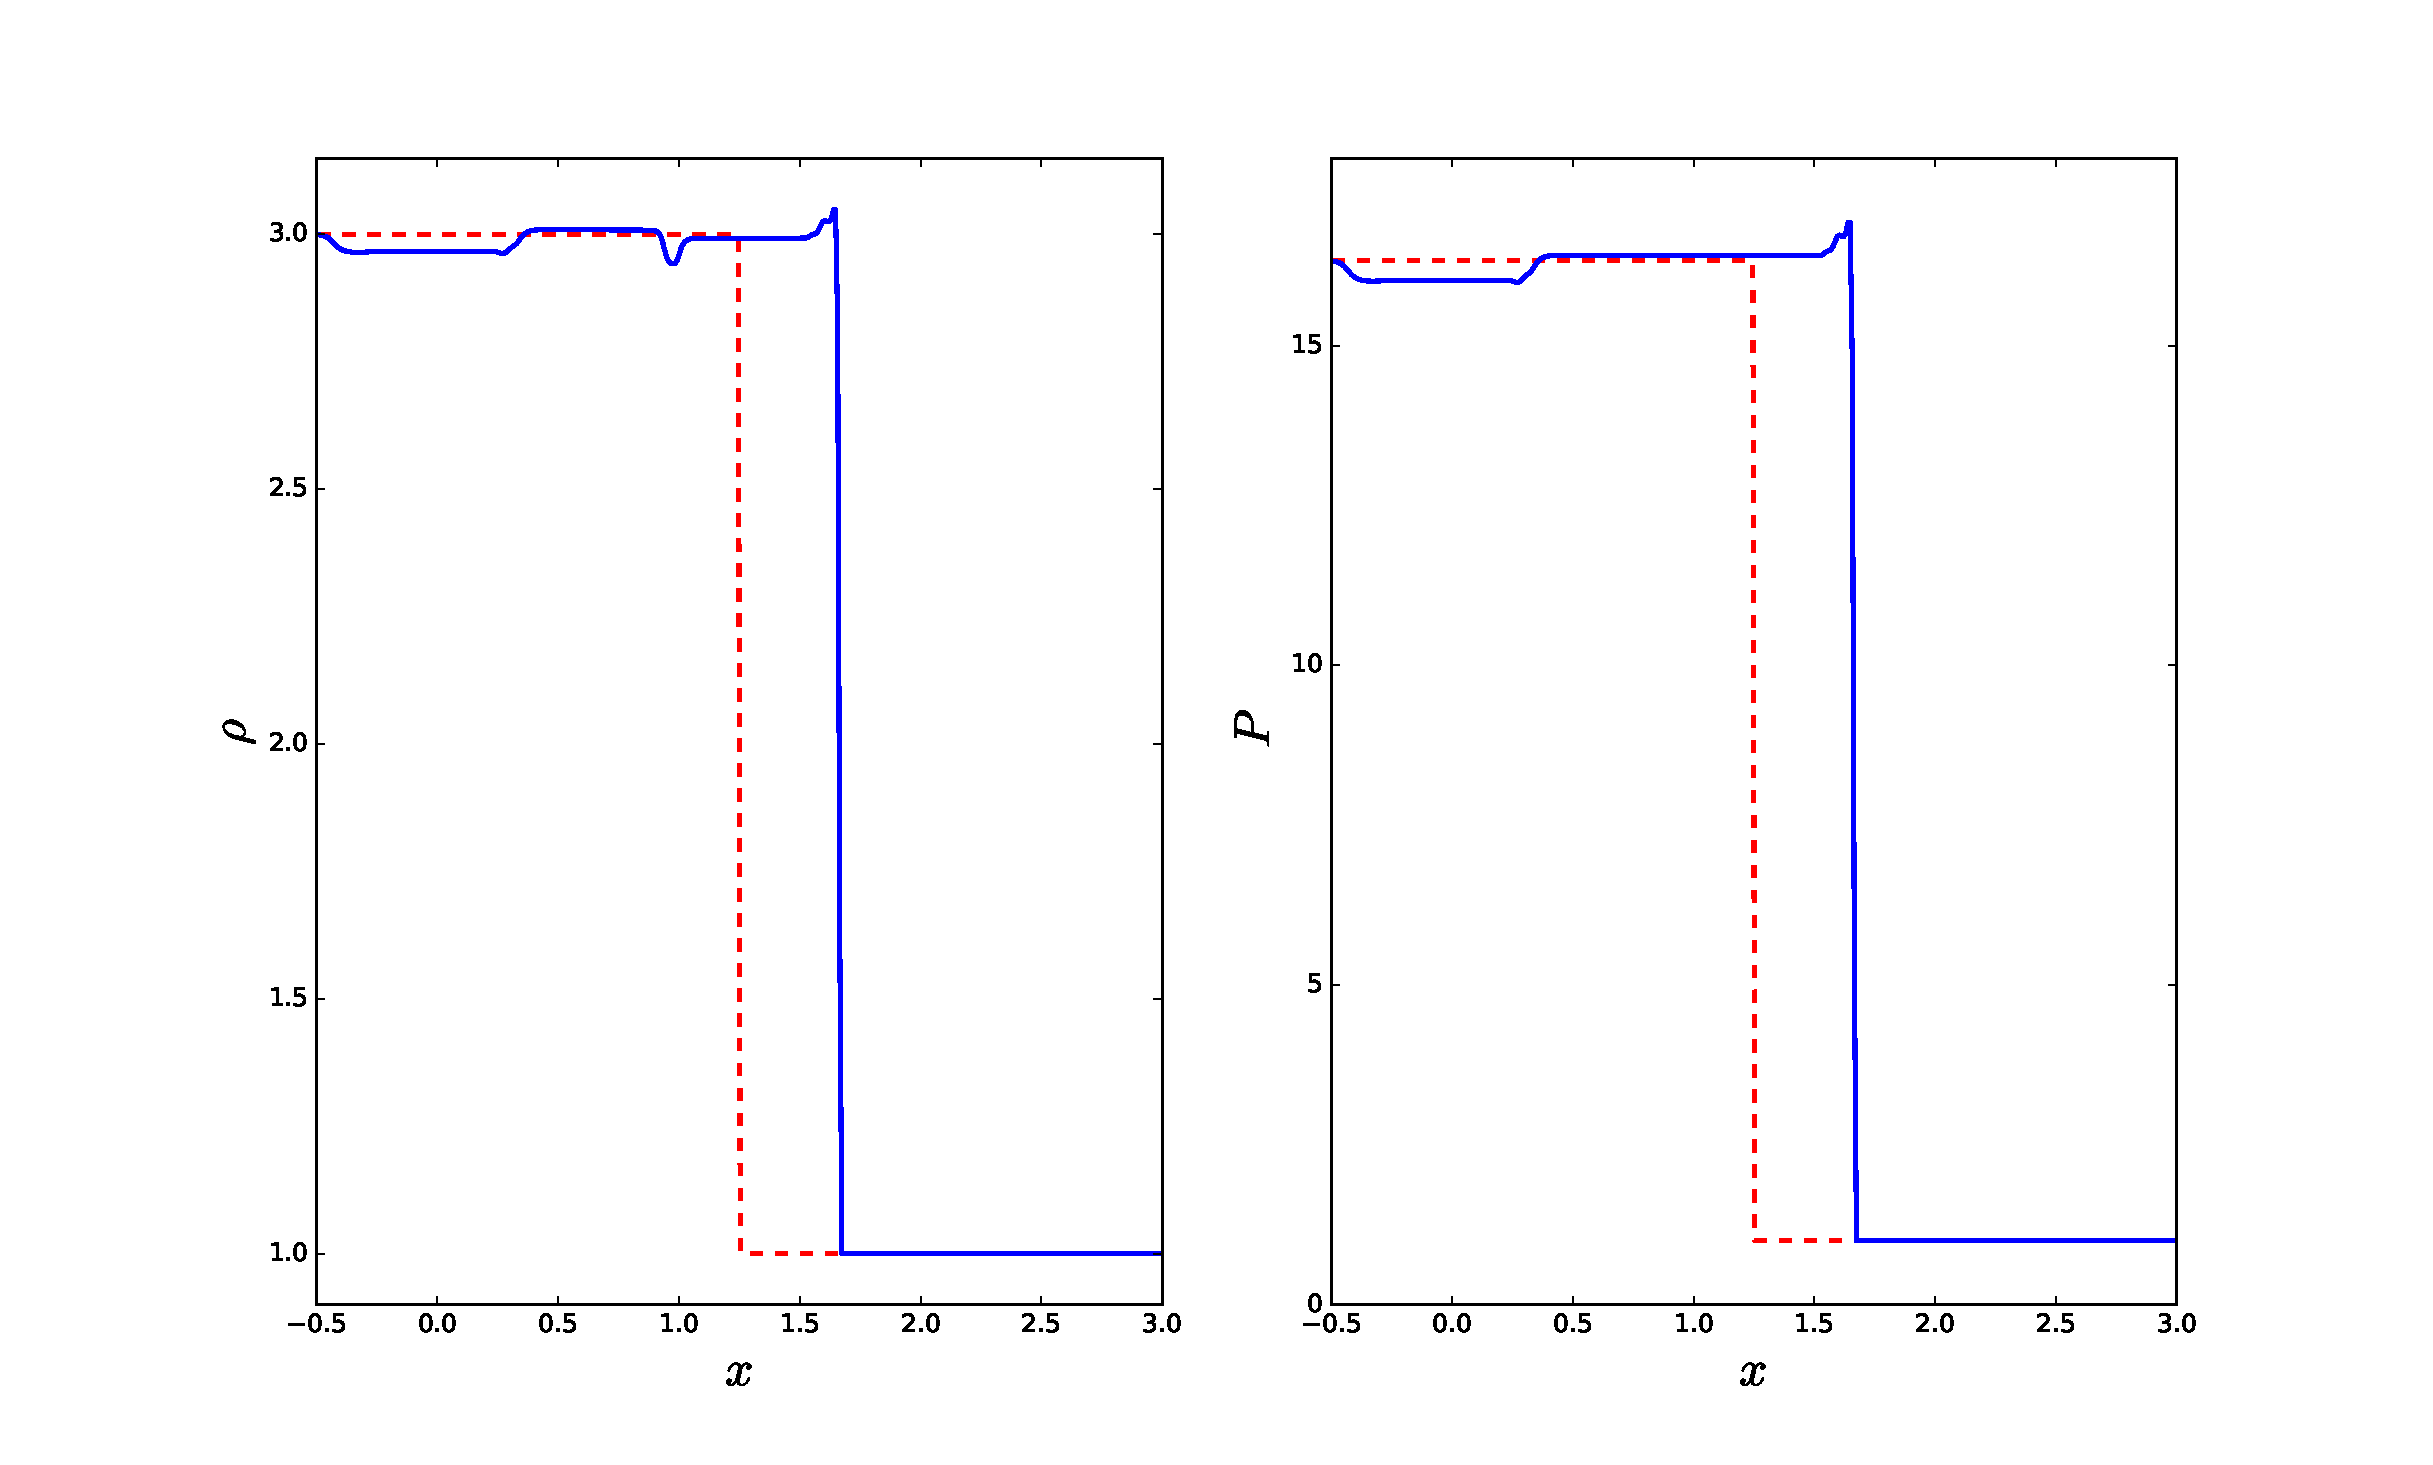
\includegraphics[width=1\textwidth]{FS1.eps}
	\end{minipage}%
\end{figure}
}
\only<2>{
\begin{figure}[ht]
	\centering
	\begin{minipage}[c]{1\textwidth}
		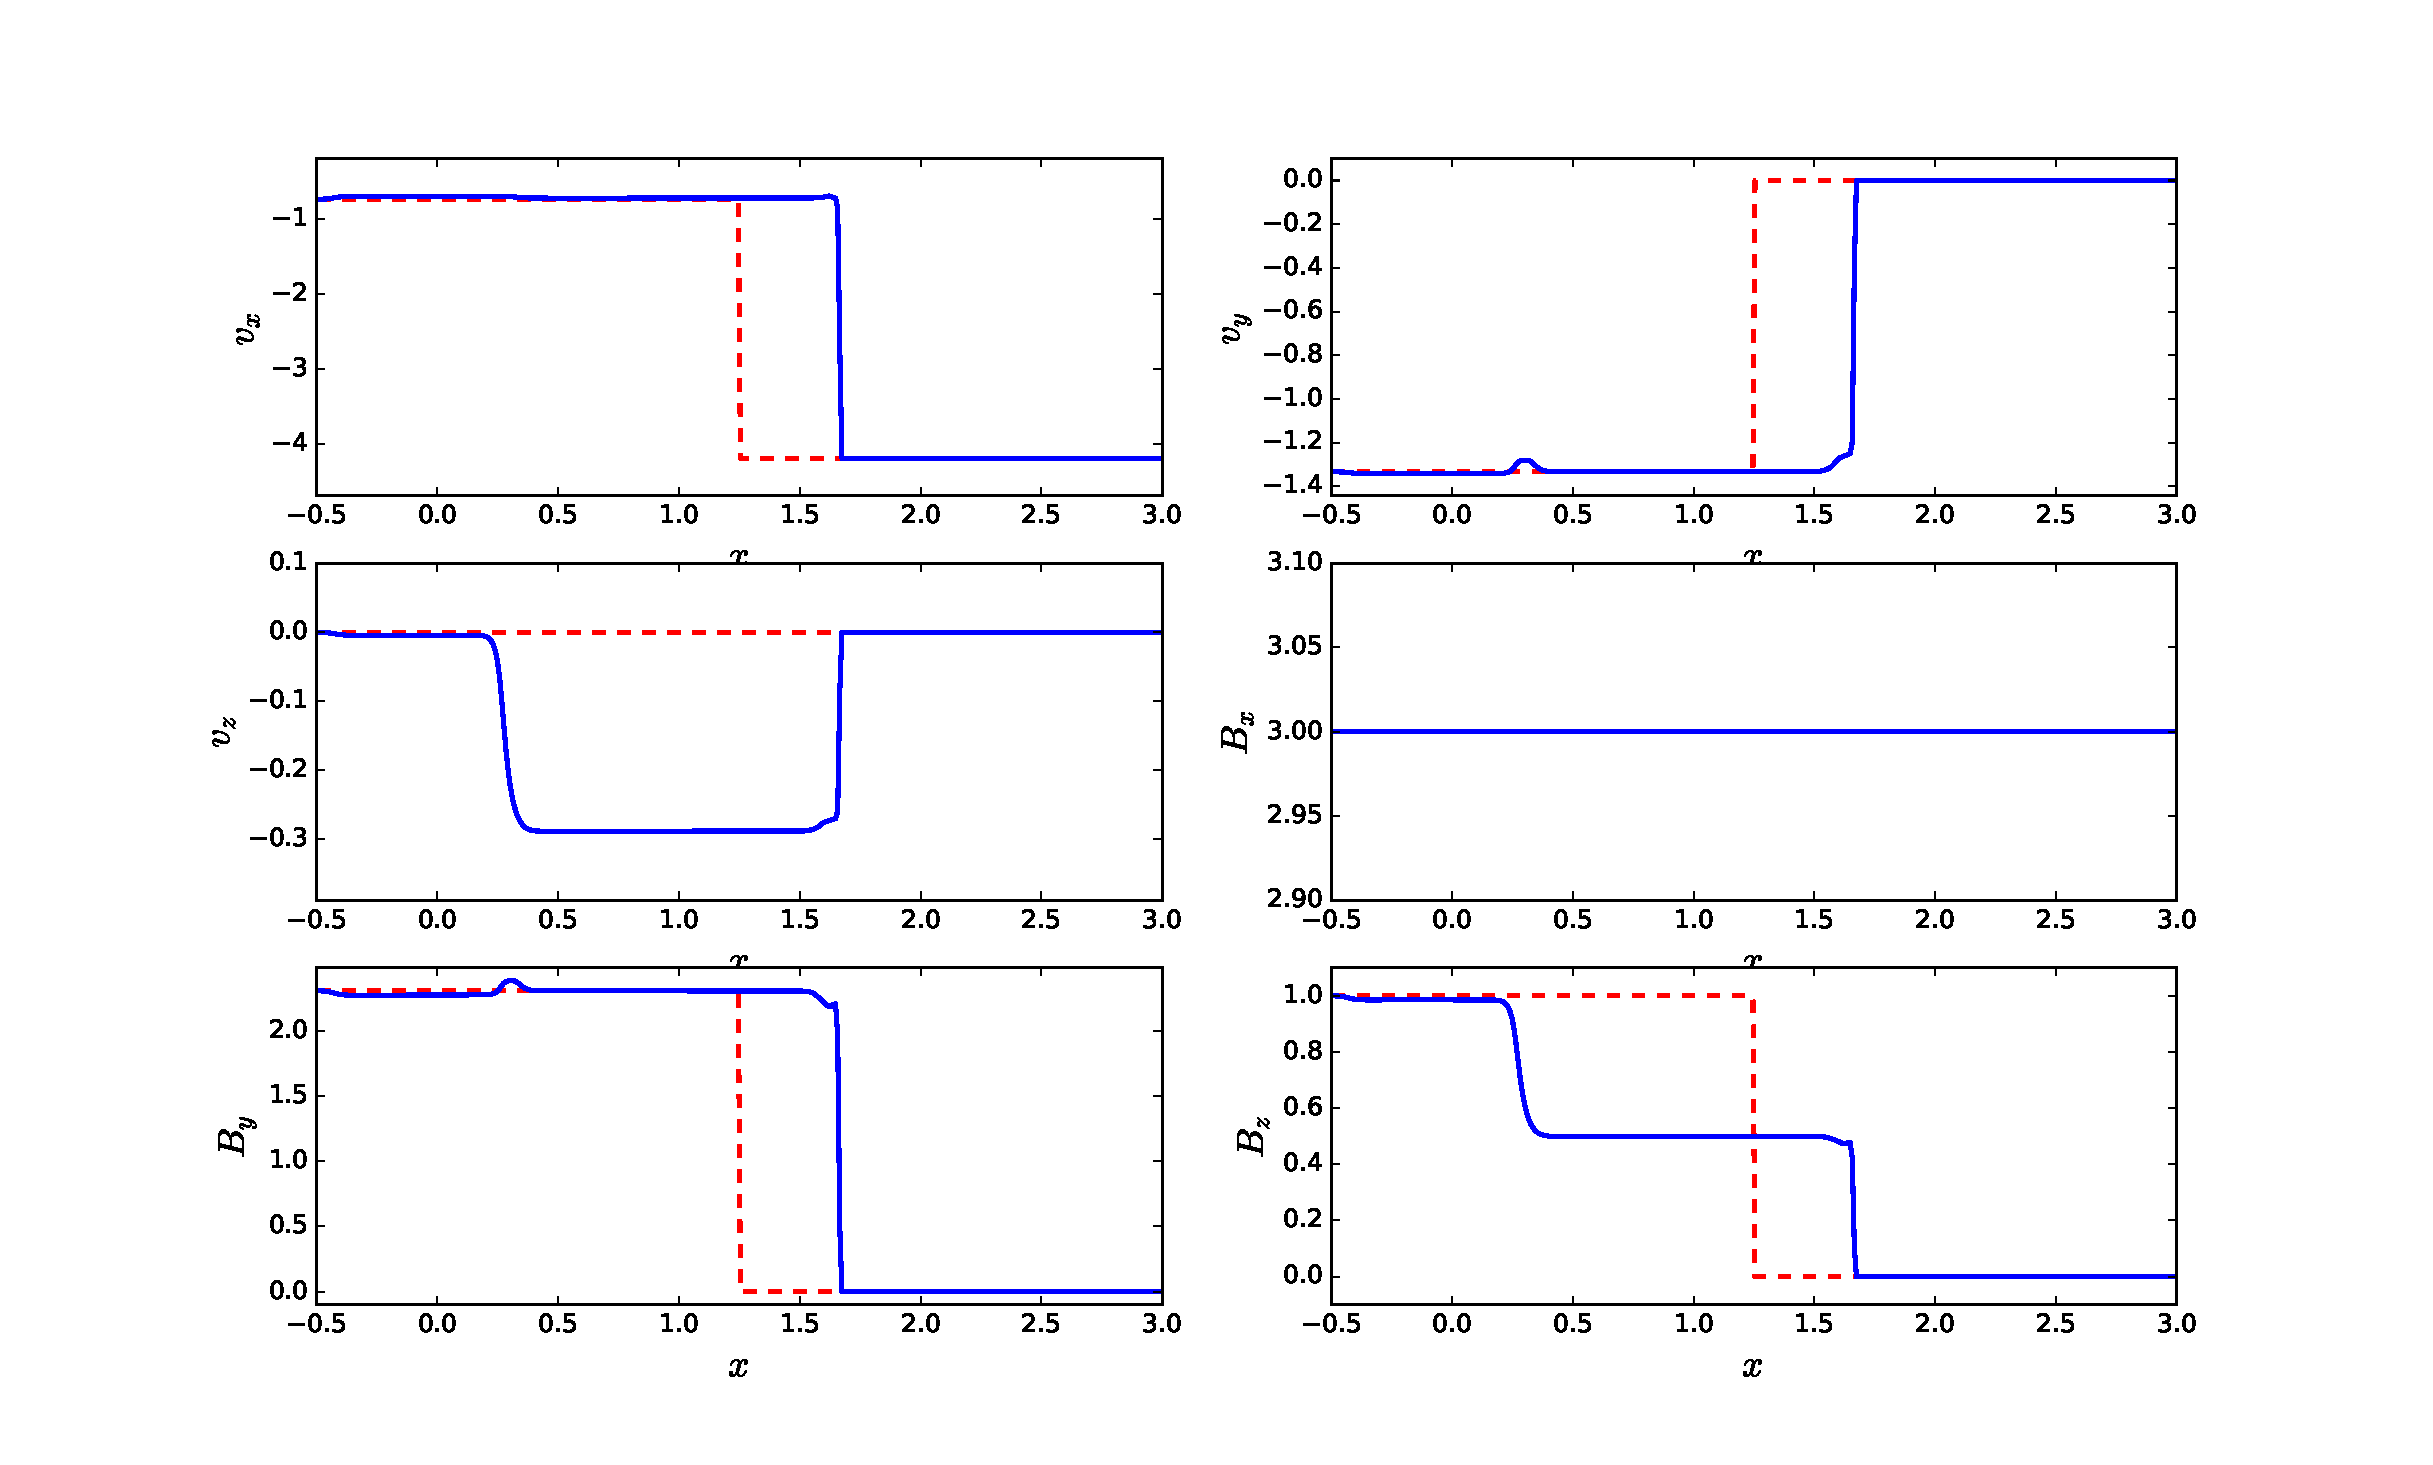
\includegraphics[width=1\textwidth]{FS2.eps}
	\end{minipage}%
\end{figure}
}
\tiny{$t_{\text{final}} =0.4$}
\end{frame}

\begin{frame}{Slow Switch-on (SS) shock test}
\only<1>{
\begin{figure}[ht]
	\centering
	\begin{minipage}[c]{1\textwidth}
		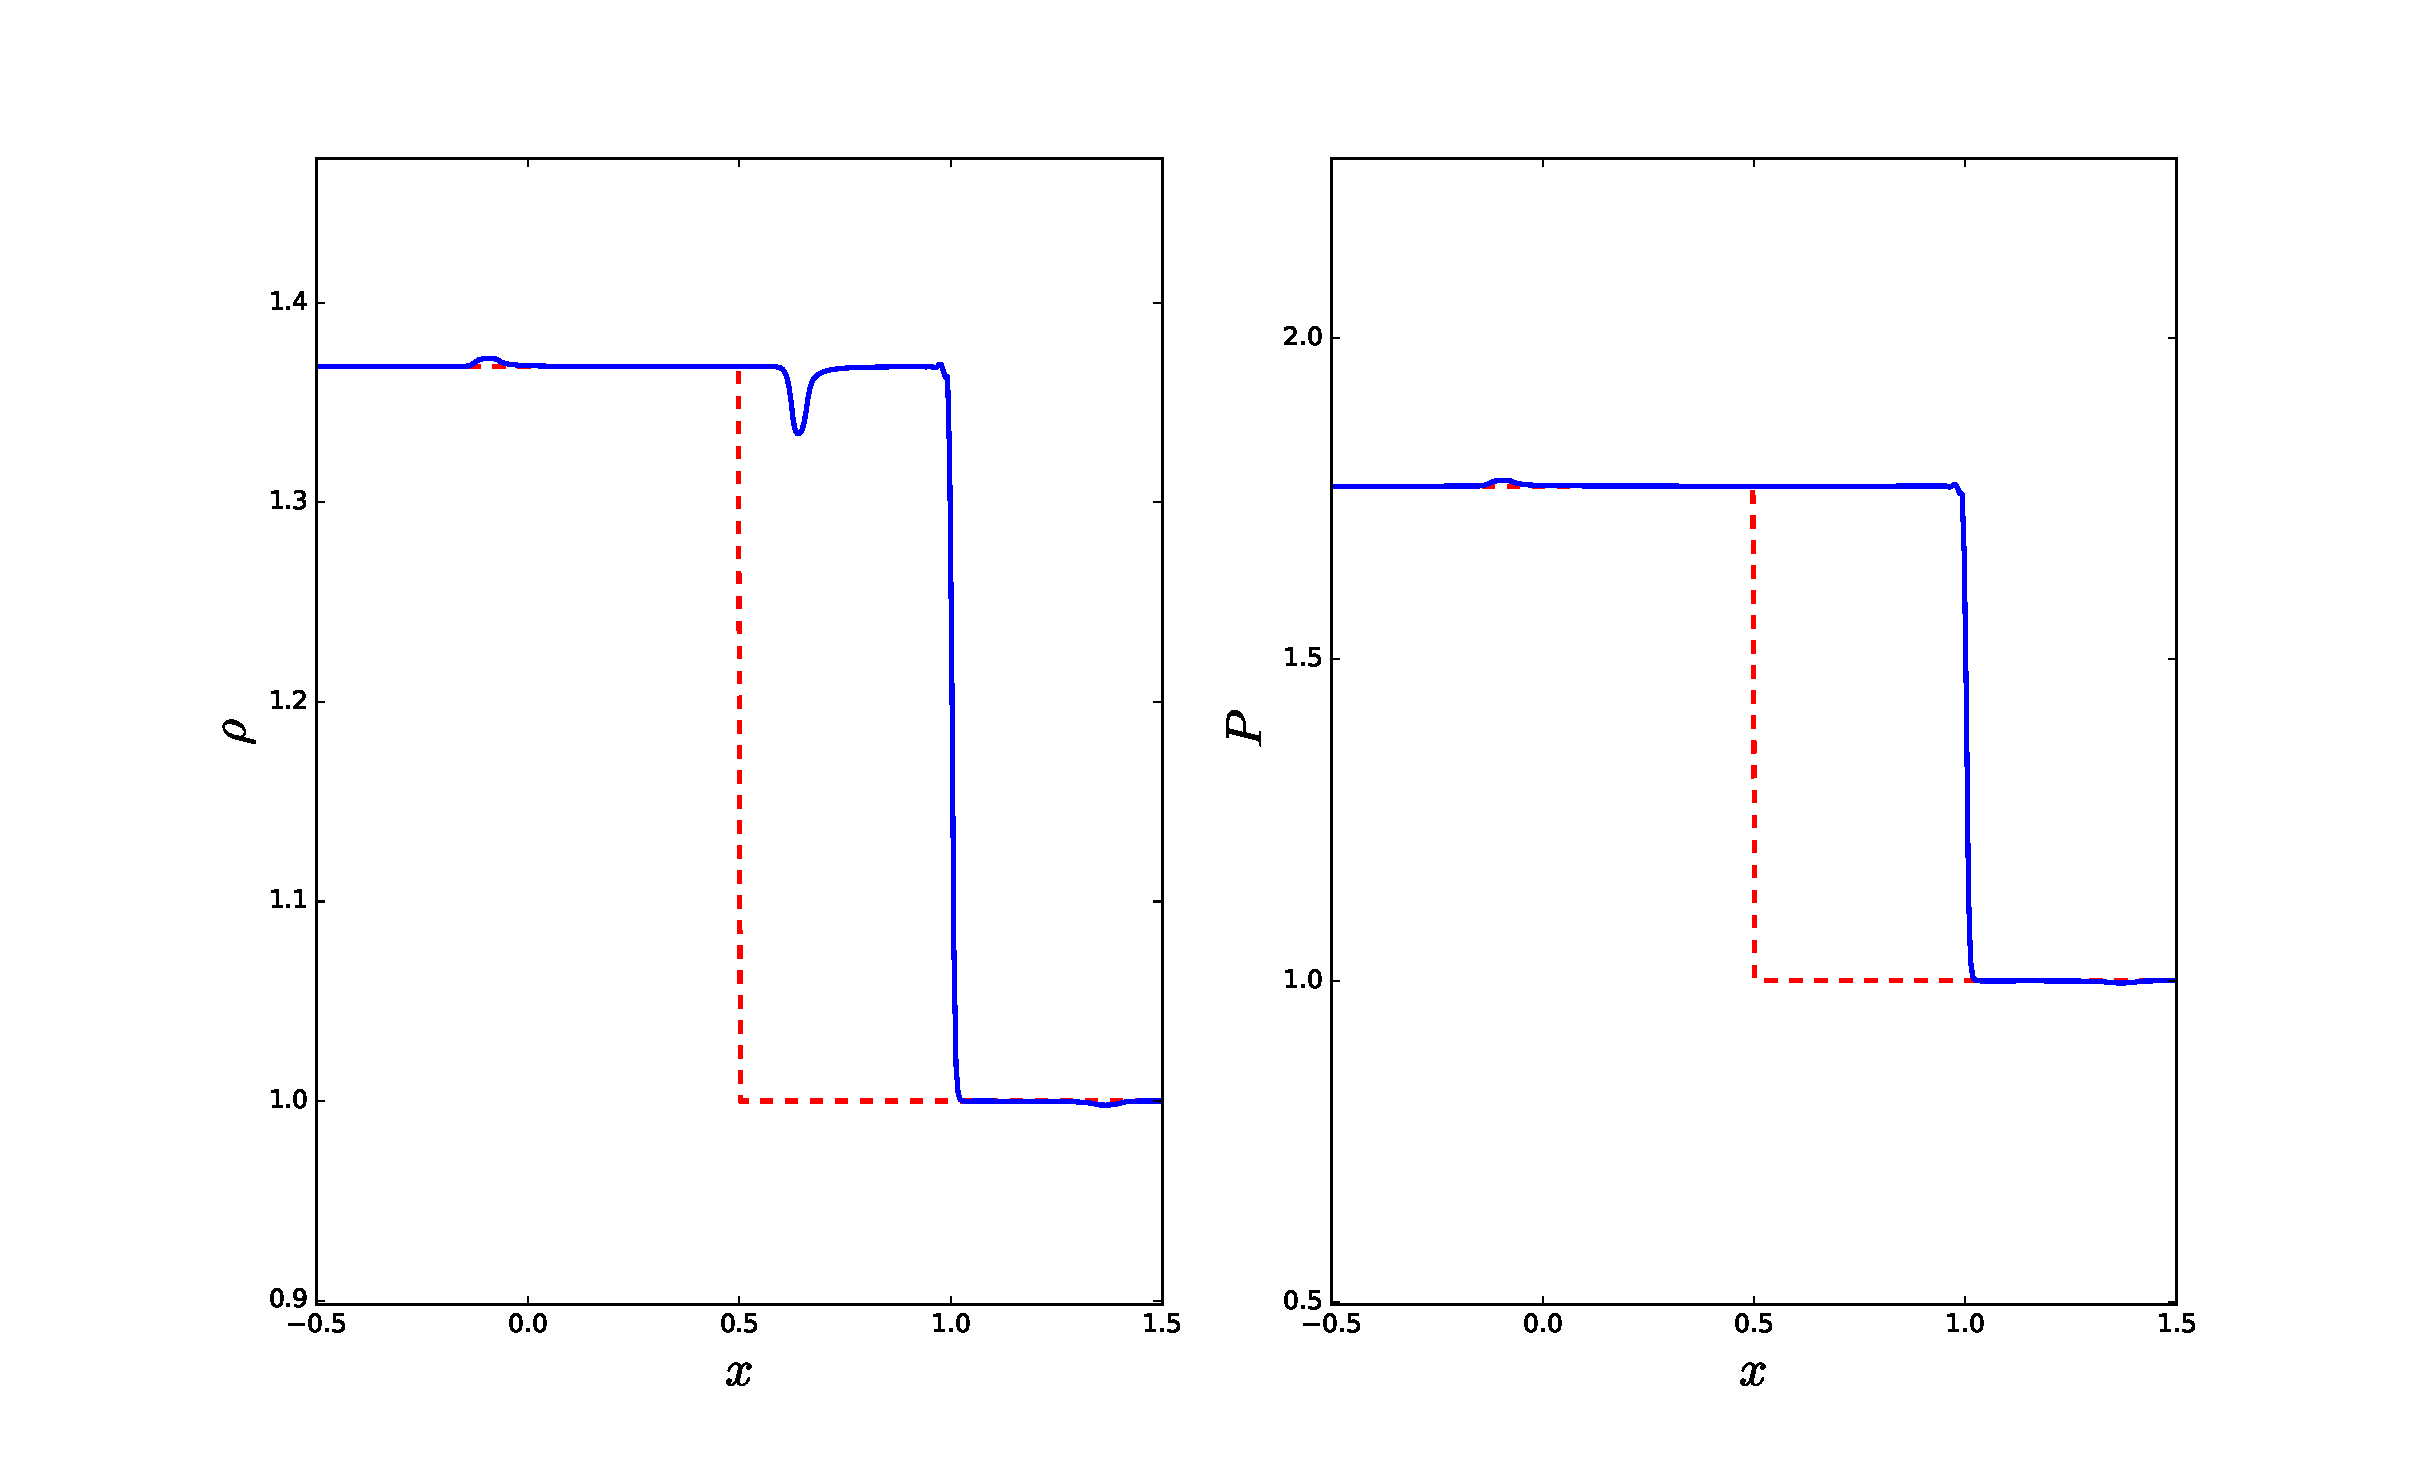
\includegraphics[width=1\textwidth]{SS1.eps}
	\end{minipage}%
\end{figure}
}
\only<2>{
\begin{figure}[ht]
	\centering
	\begin{minipage}[c]{1\textwidth}
		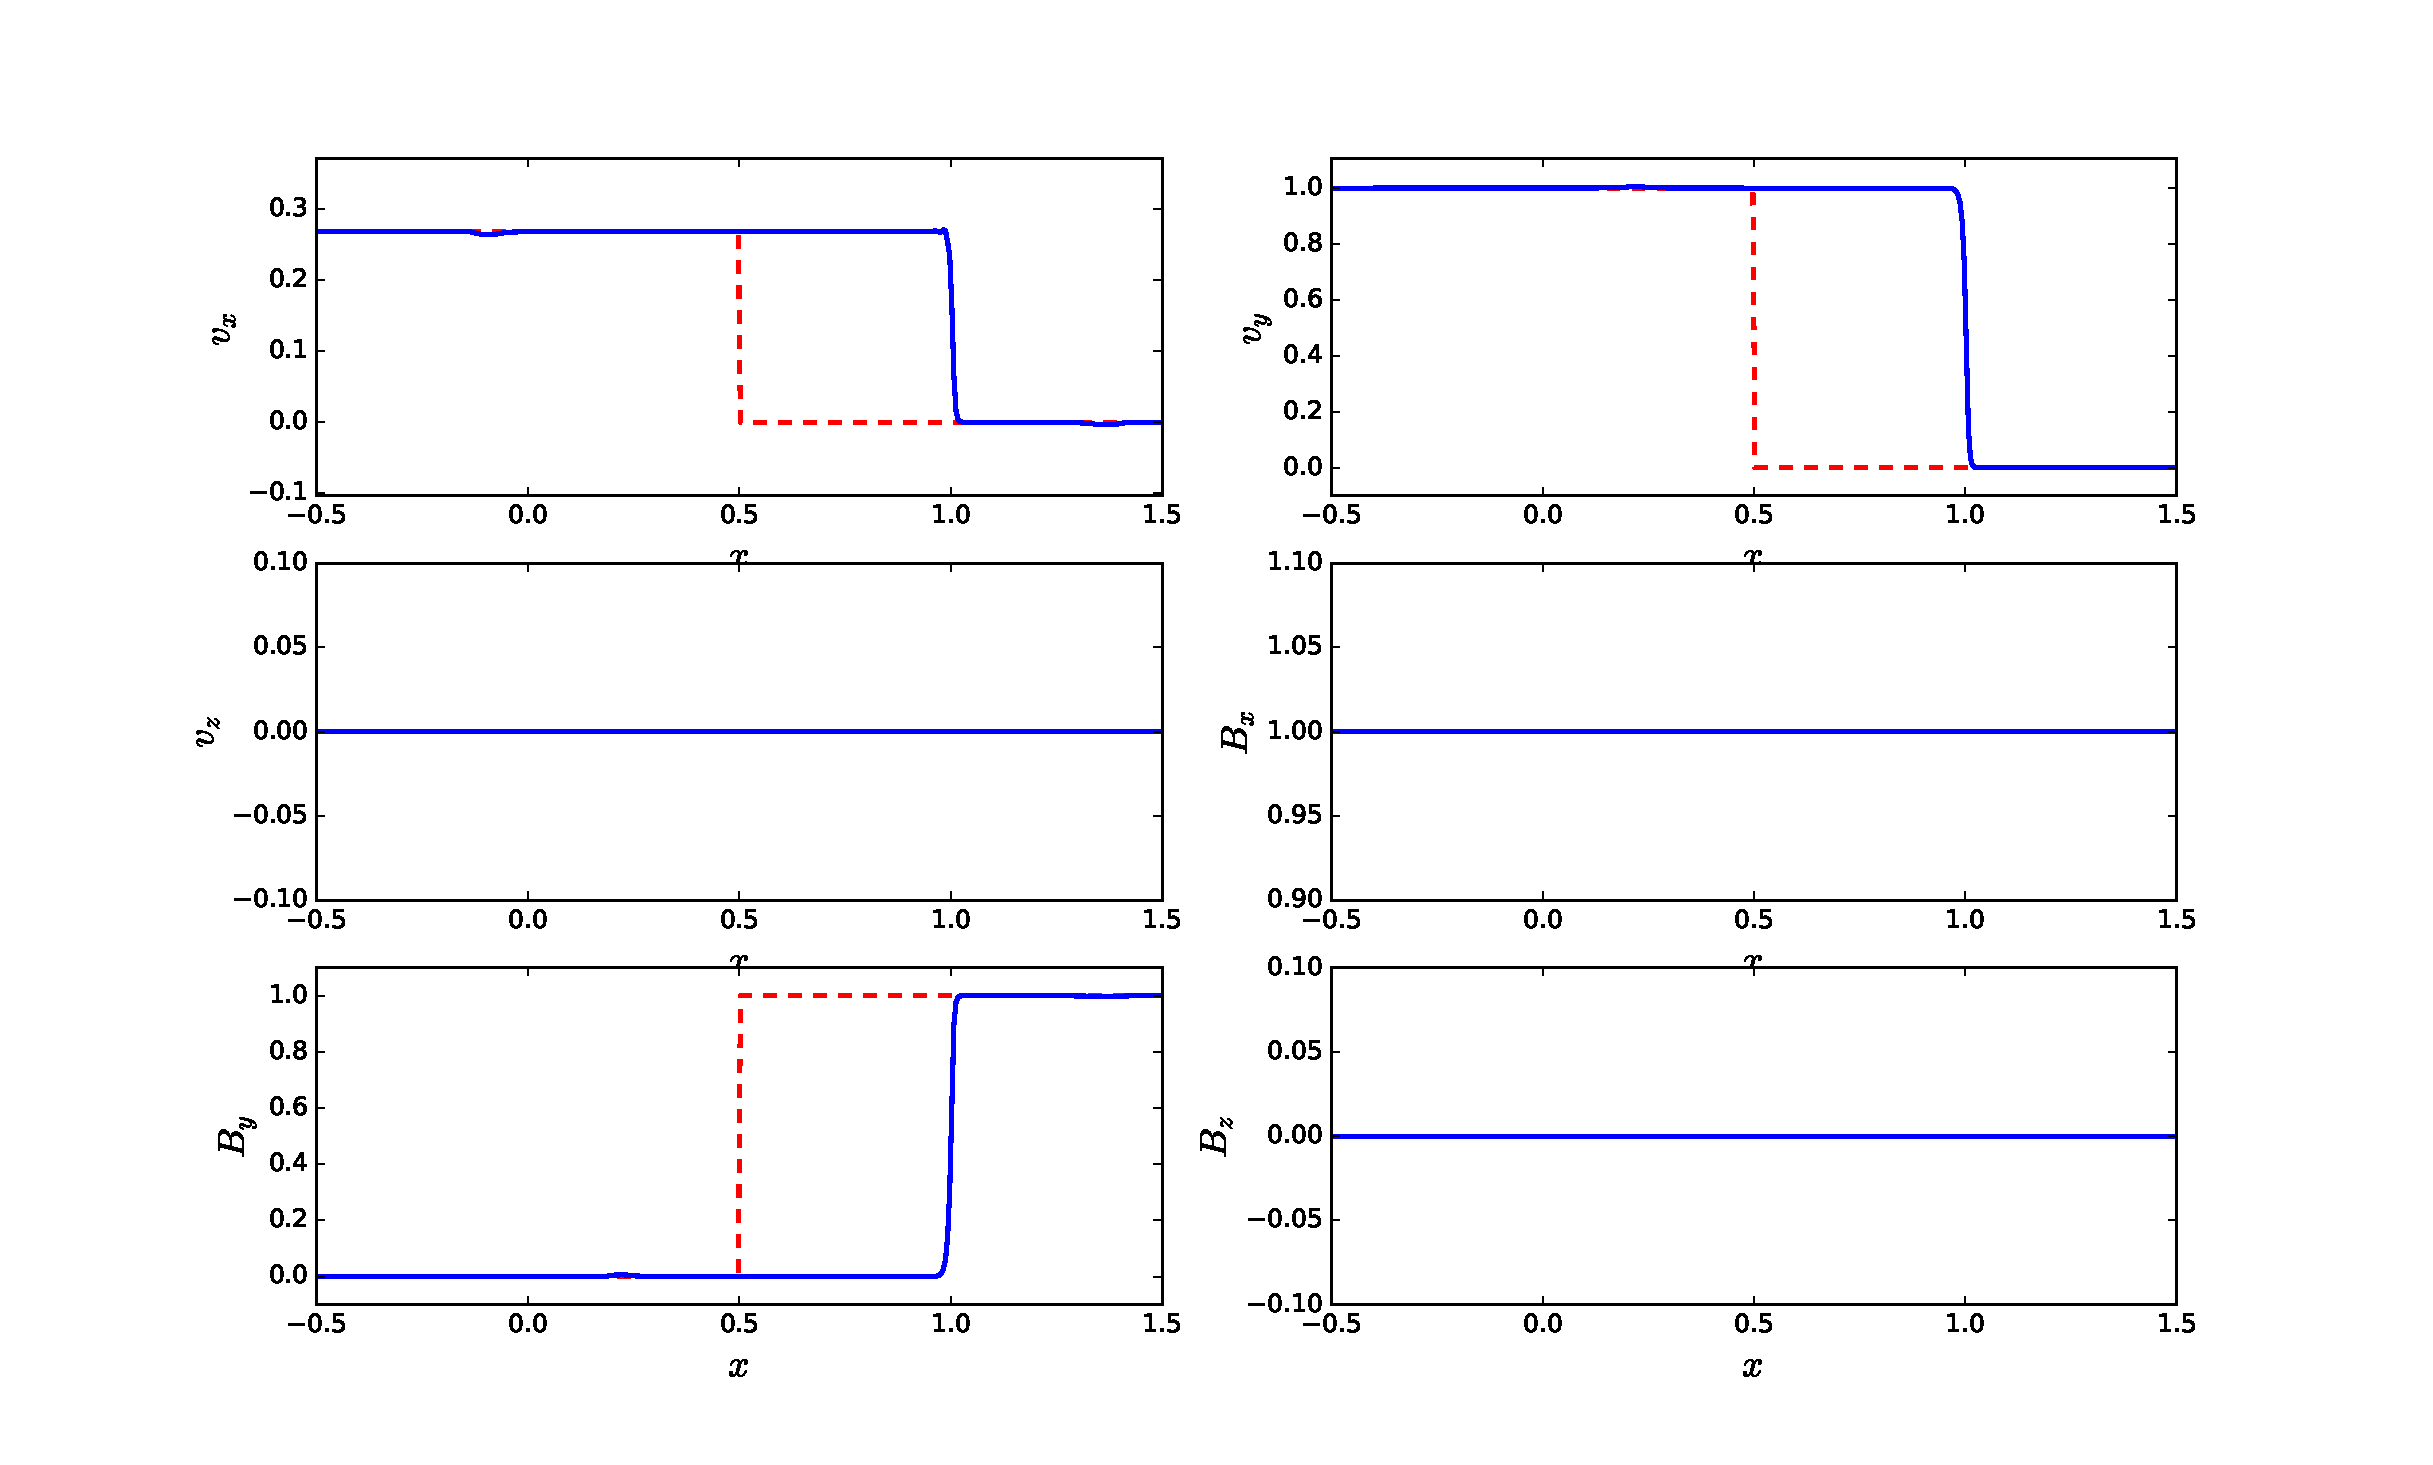
\includegraphics[width=1\textwidth]{SS2.eps}
	\end{minipage}%
\end{figure}
}
\tiny{$t_{\text{final}} =0.5$}
\end{frame}

\begin{frame}{Fast Rarefaction (FR) waves test}
\only<1>{
\begin{figure}[ht]
	\centering
	\begin{minipage}[c]{1\textwidth}
		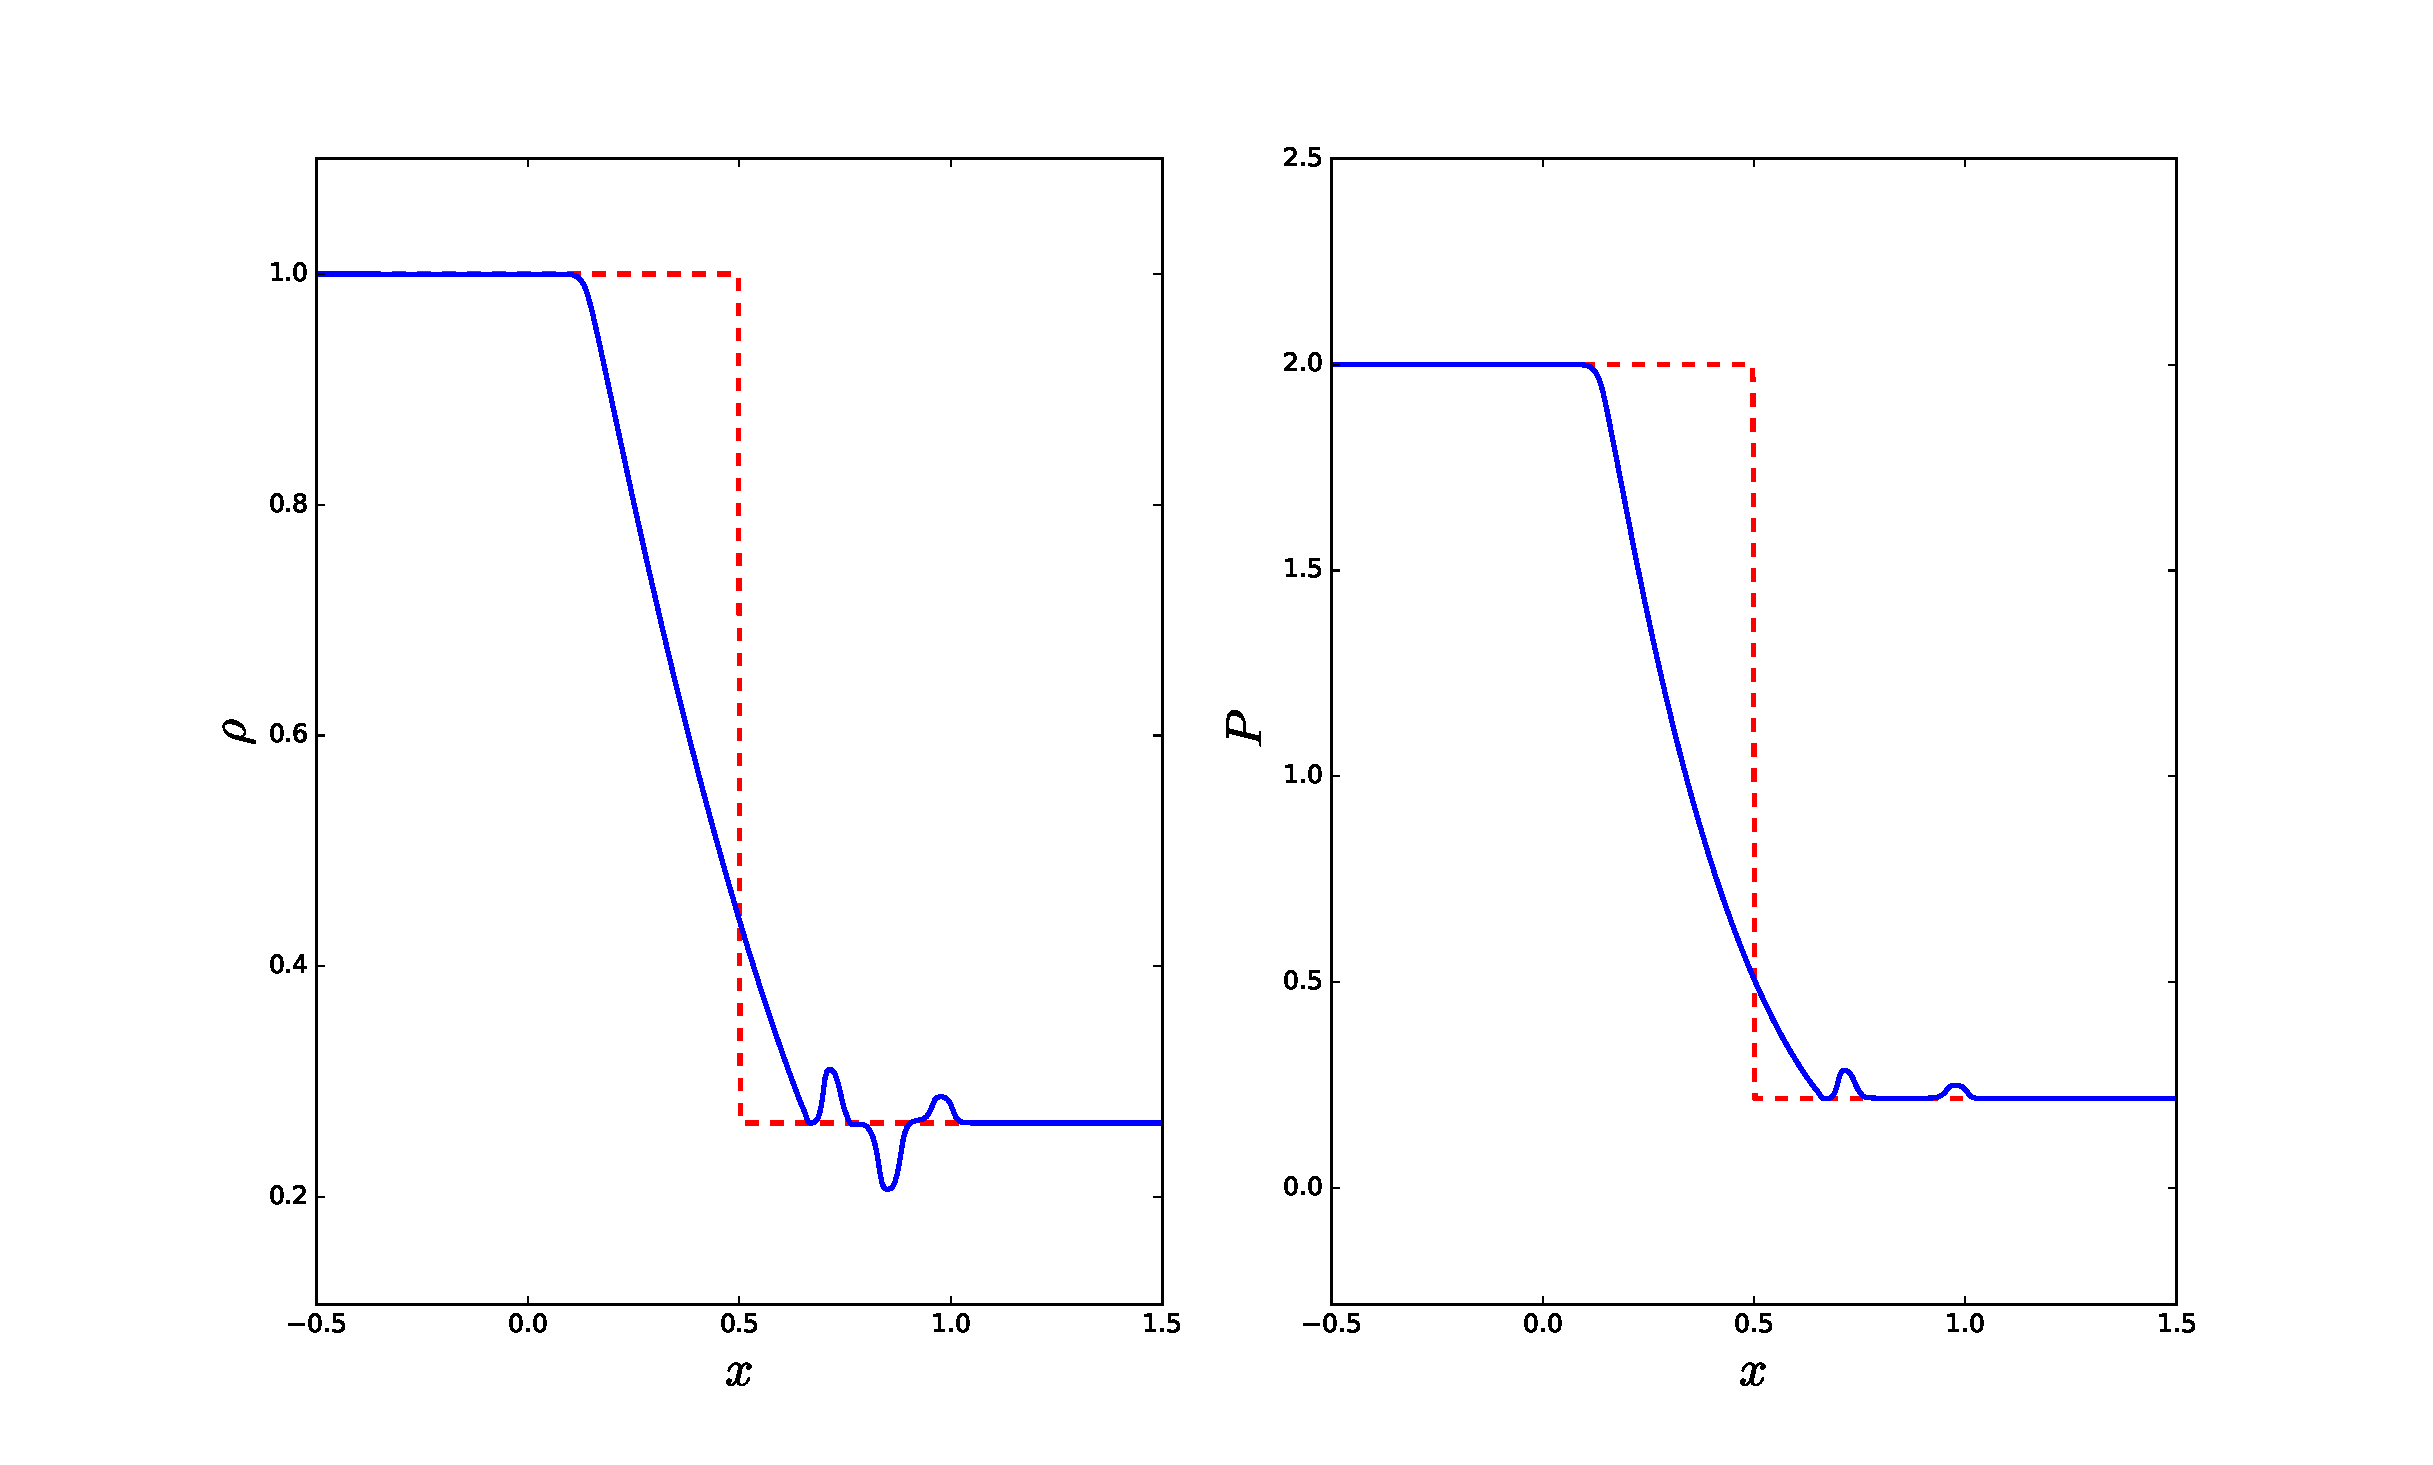
\includegraphics[width=1\textwidth]{FR1.eps}
	\end{minipage}%
\end{figure}
}
\only<2>{
\begin{figure}[ht]
	\centering
	\begin{minipage}[c]{1\textwidth}
		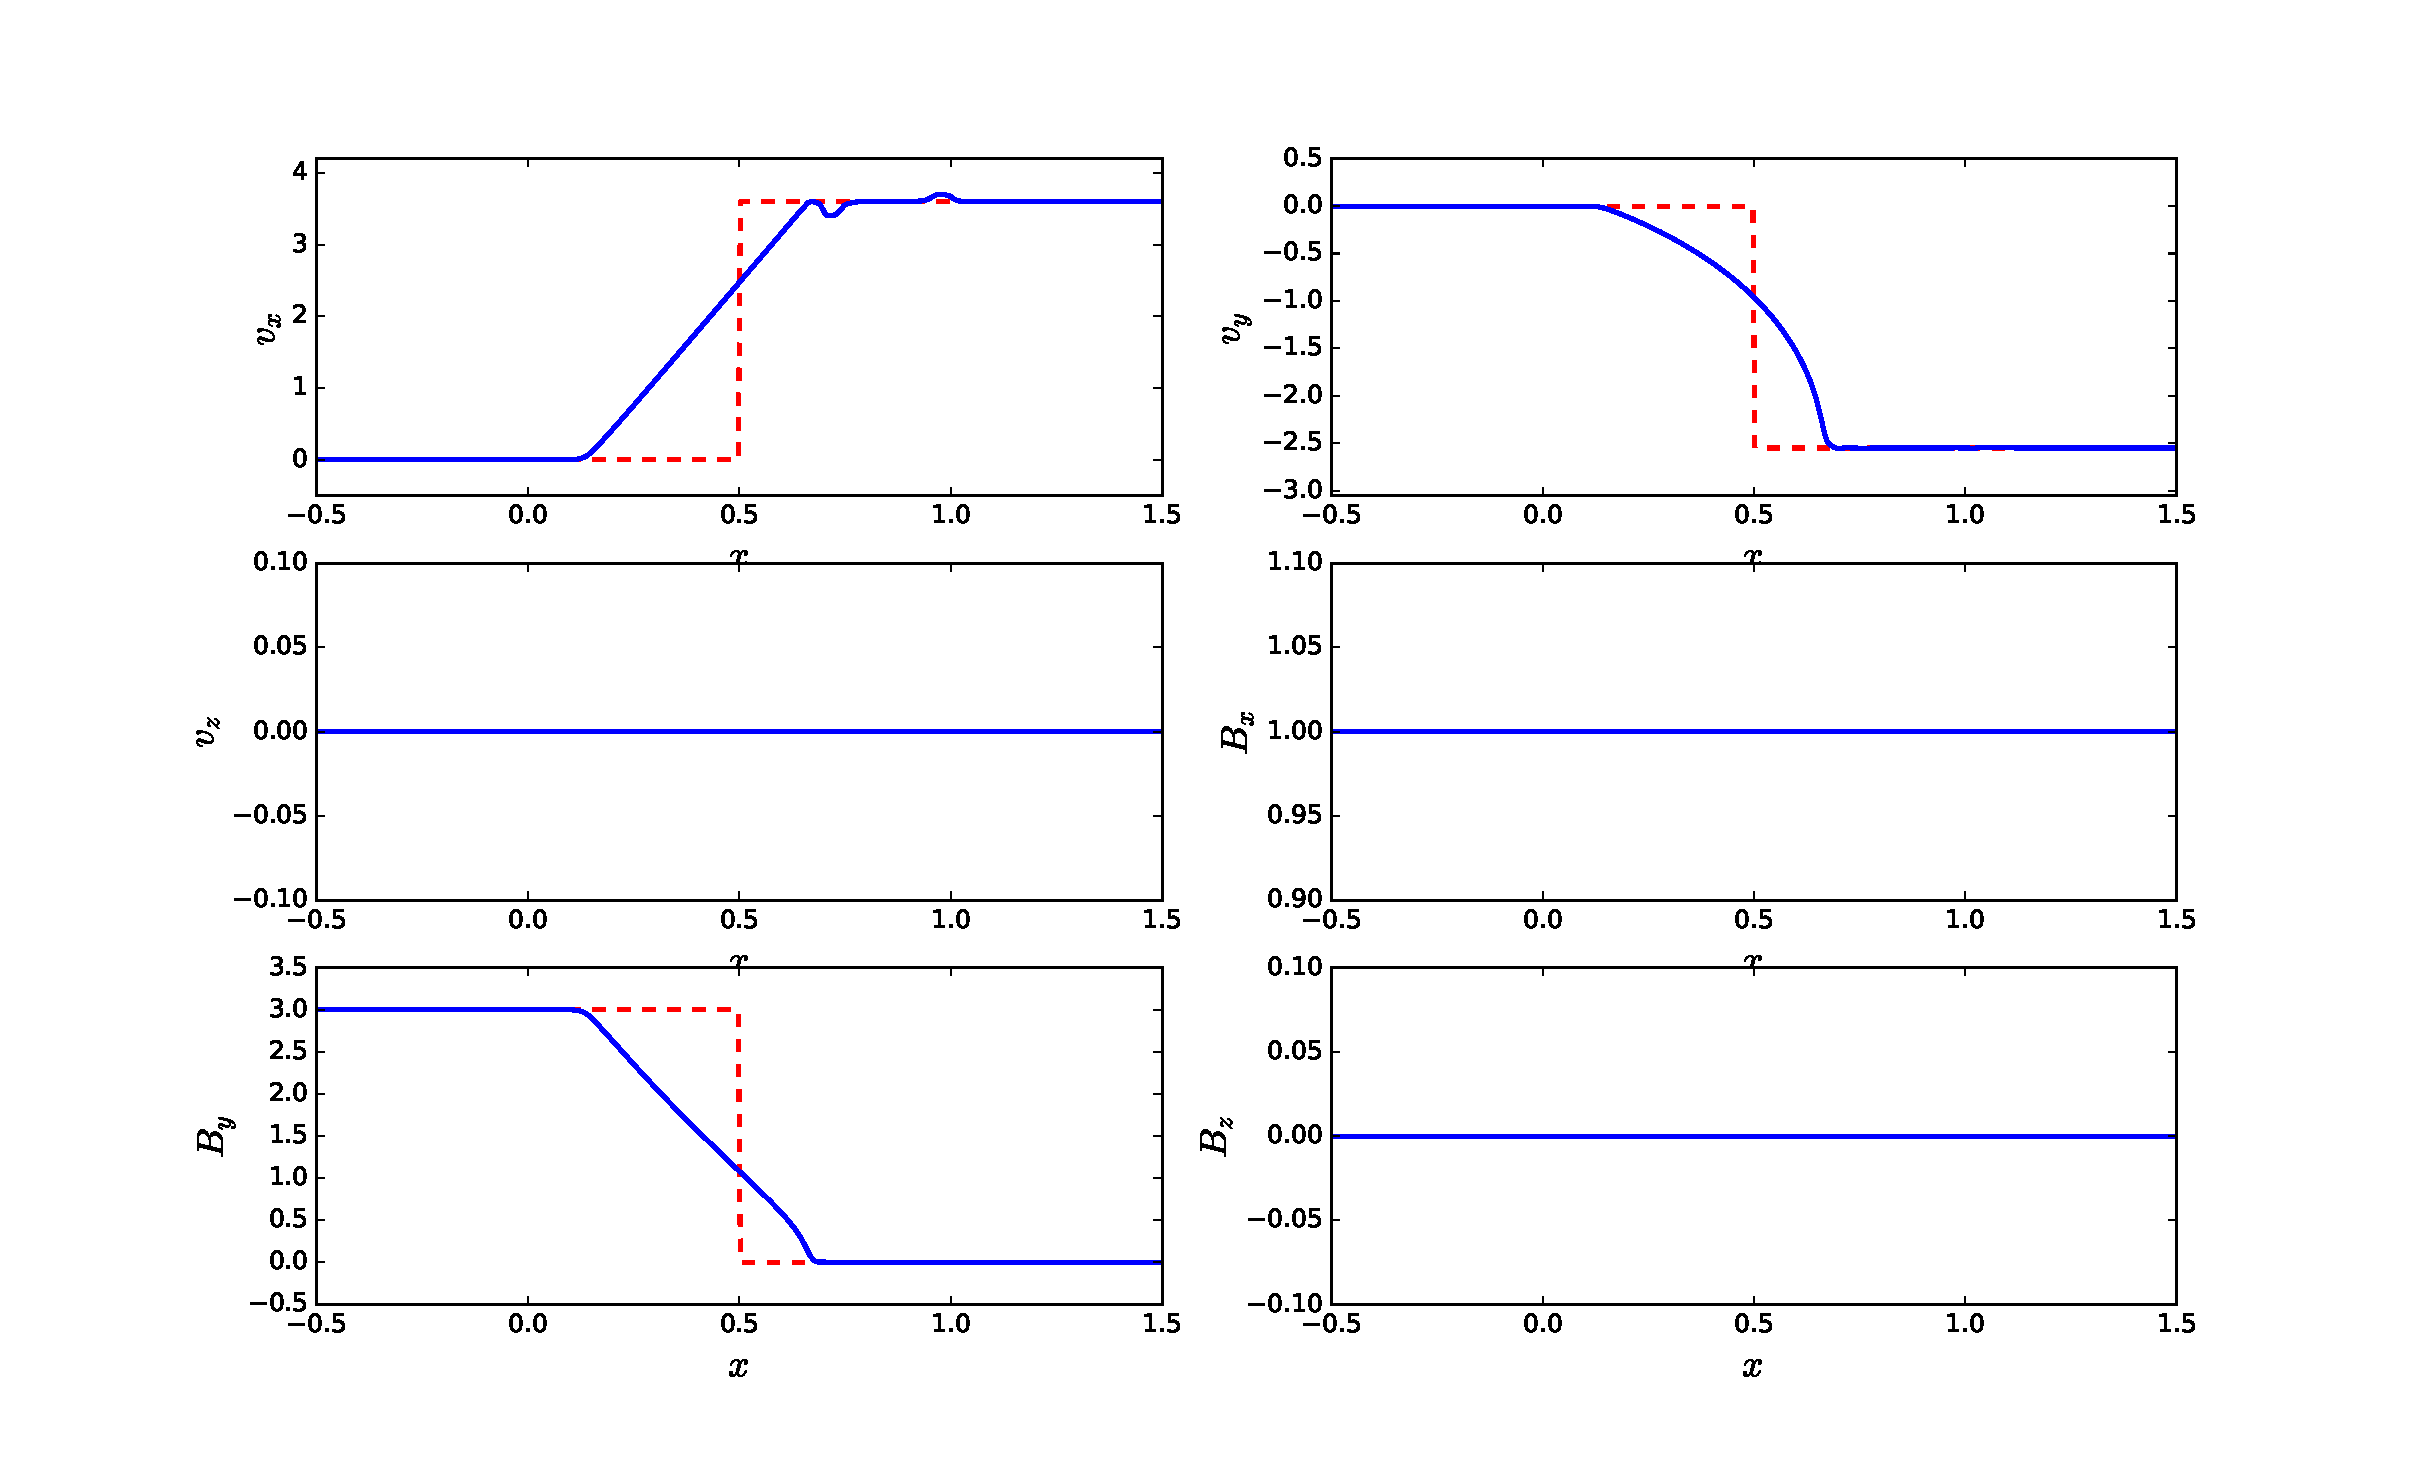
\includegraphics[width=1\textwidth]{FR2.eps}
	\end{minipage}%
\end{figure}
}
\tiny{$t_{\text{final}} =0.1$}
\end{frame}

\begin{frame}{Slow Rarefaction (SR) waves test}
\only<1>{
\begin{figure}[ht]
	\centering
	\begin{minipage}[c]{1\textwidth}
		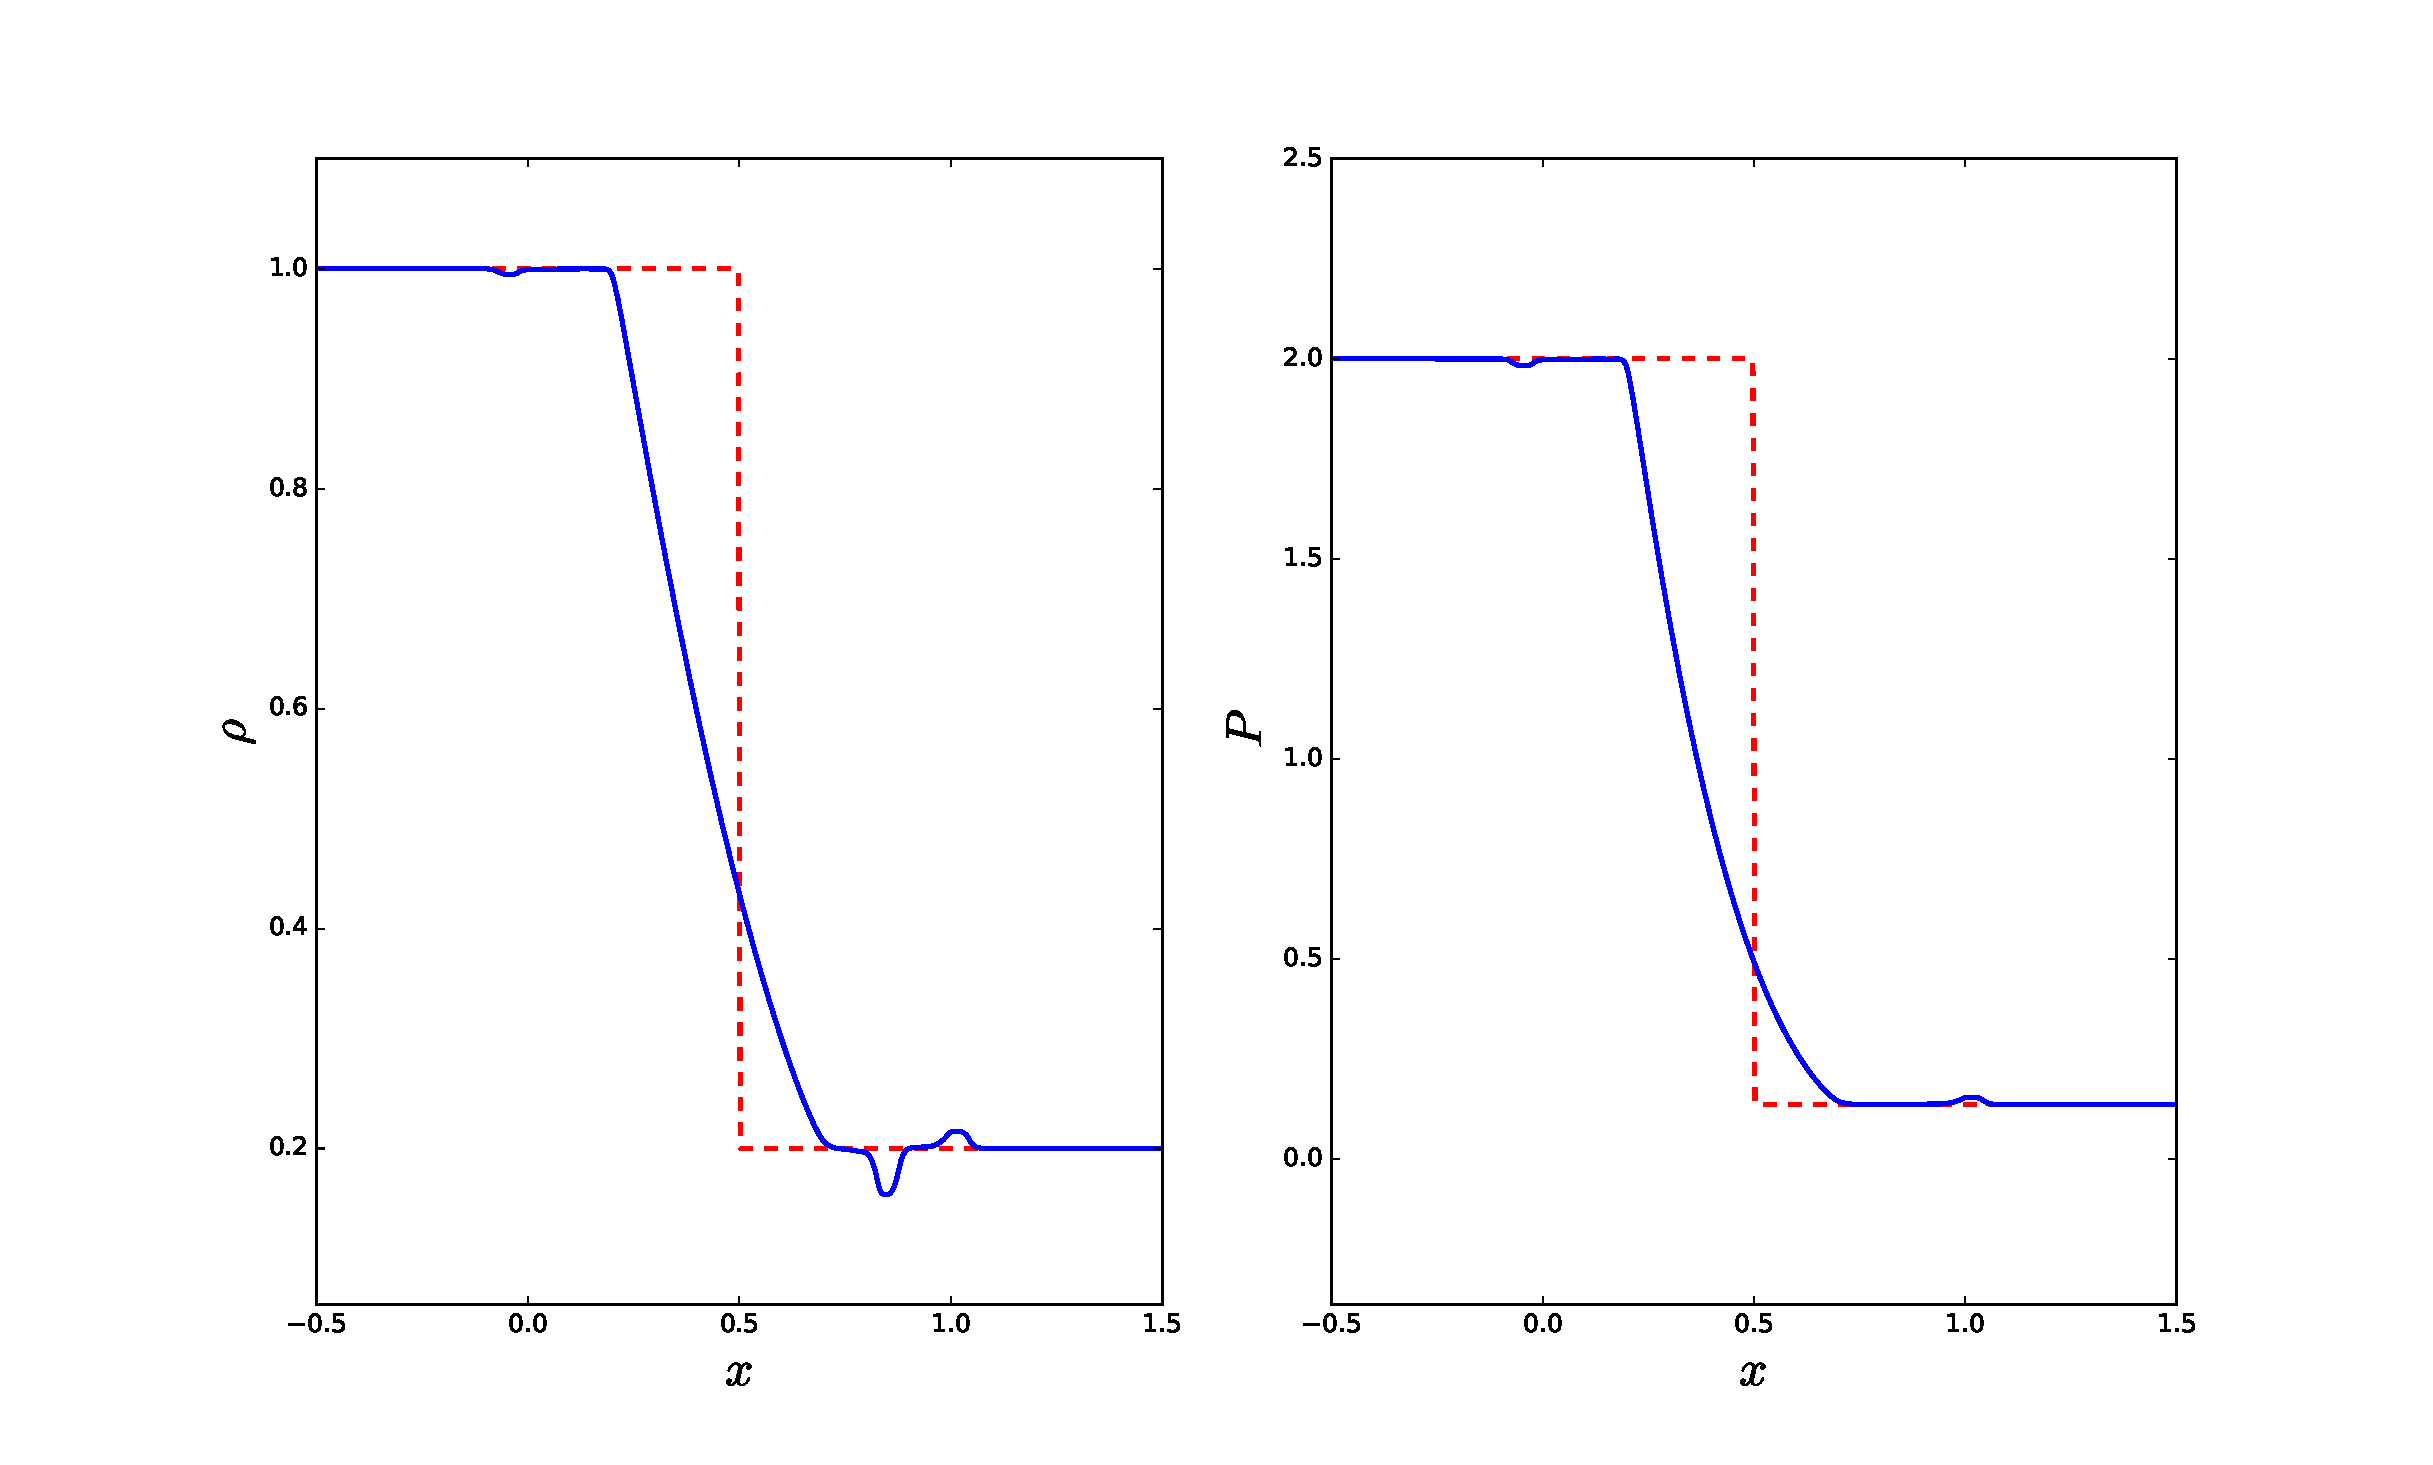
\includegraphics[width=1\textwidth]{SR1.eps}
	\end{minipage}%
\end{figure}
}
\only<2>{
\begin{figure}[ht]
	\centering
	\begin{minipage}[c]{1\textwidth}
		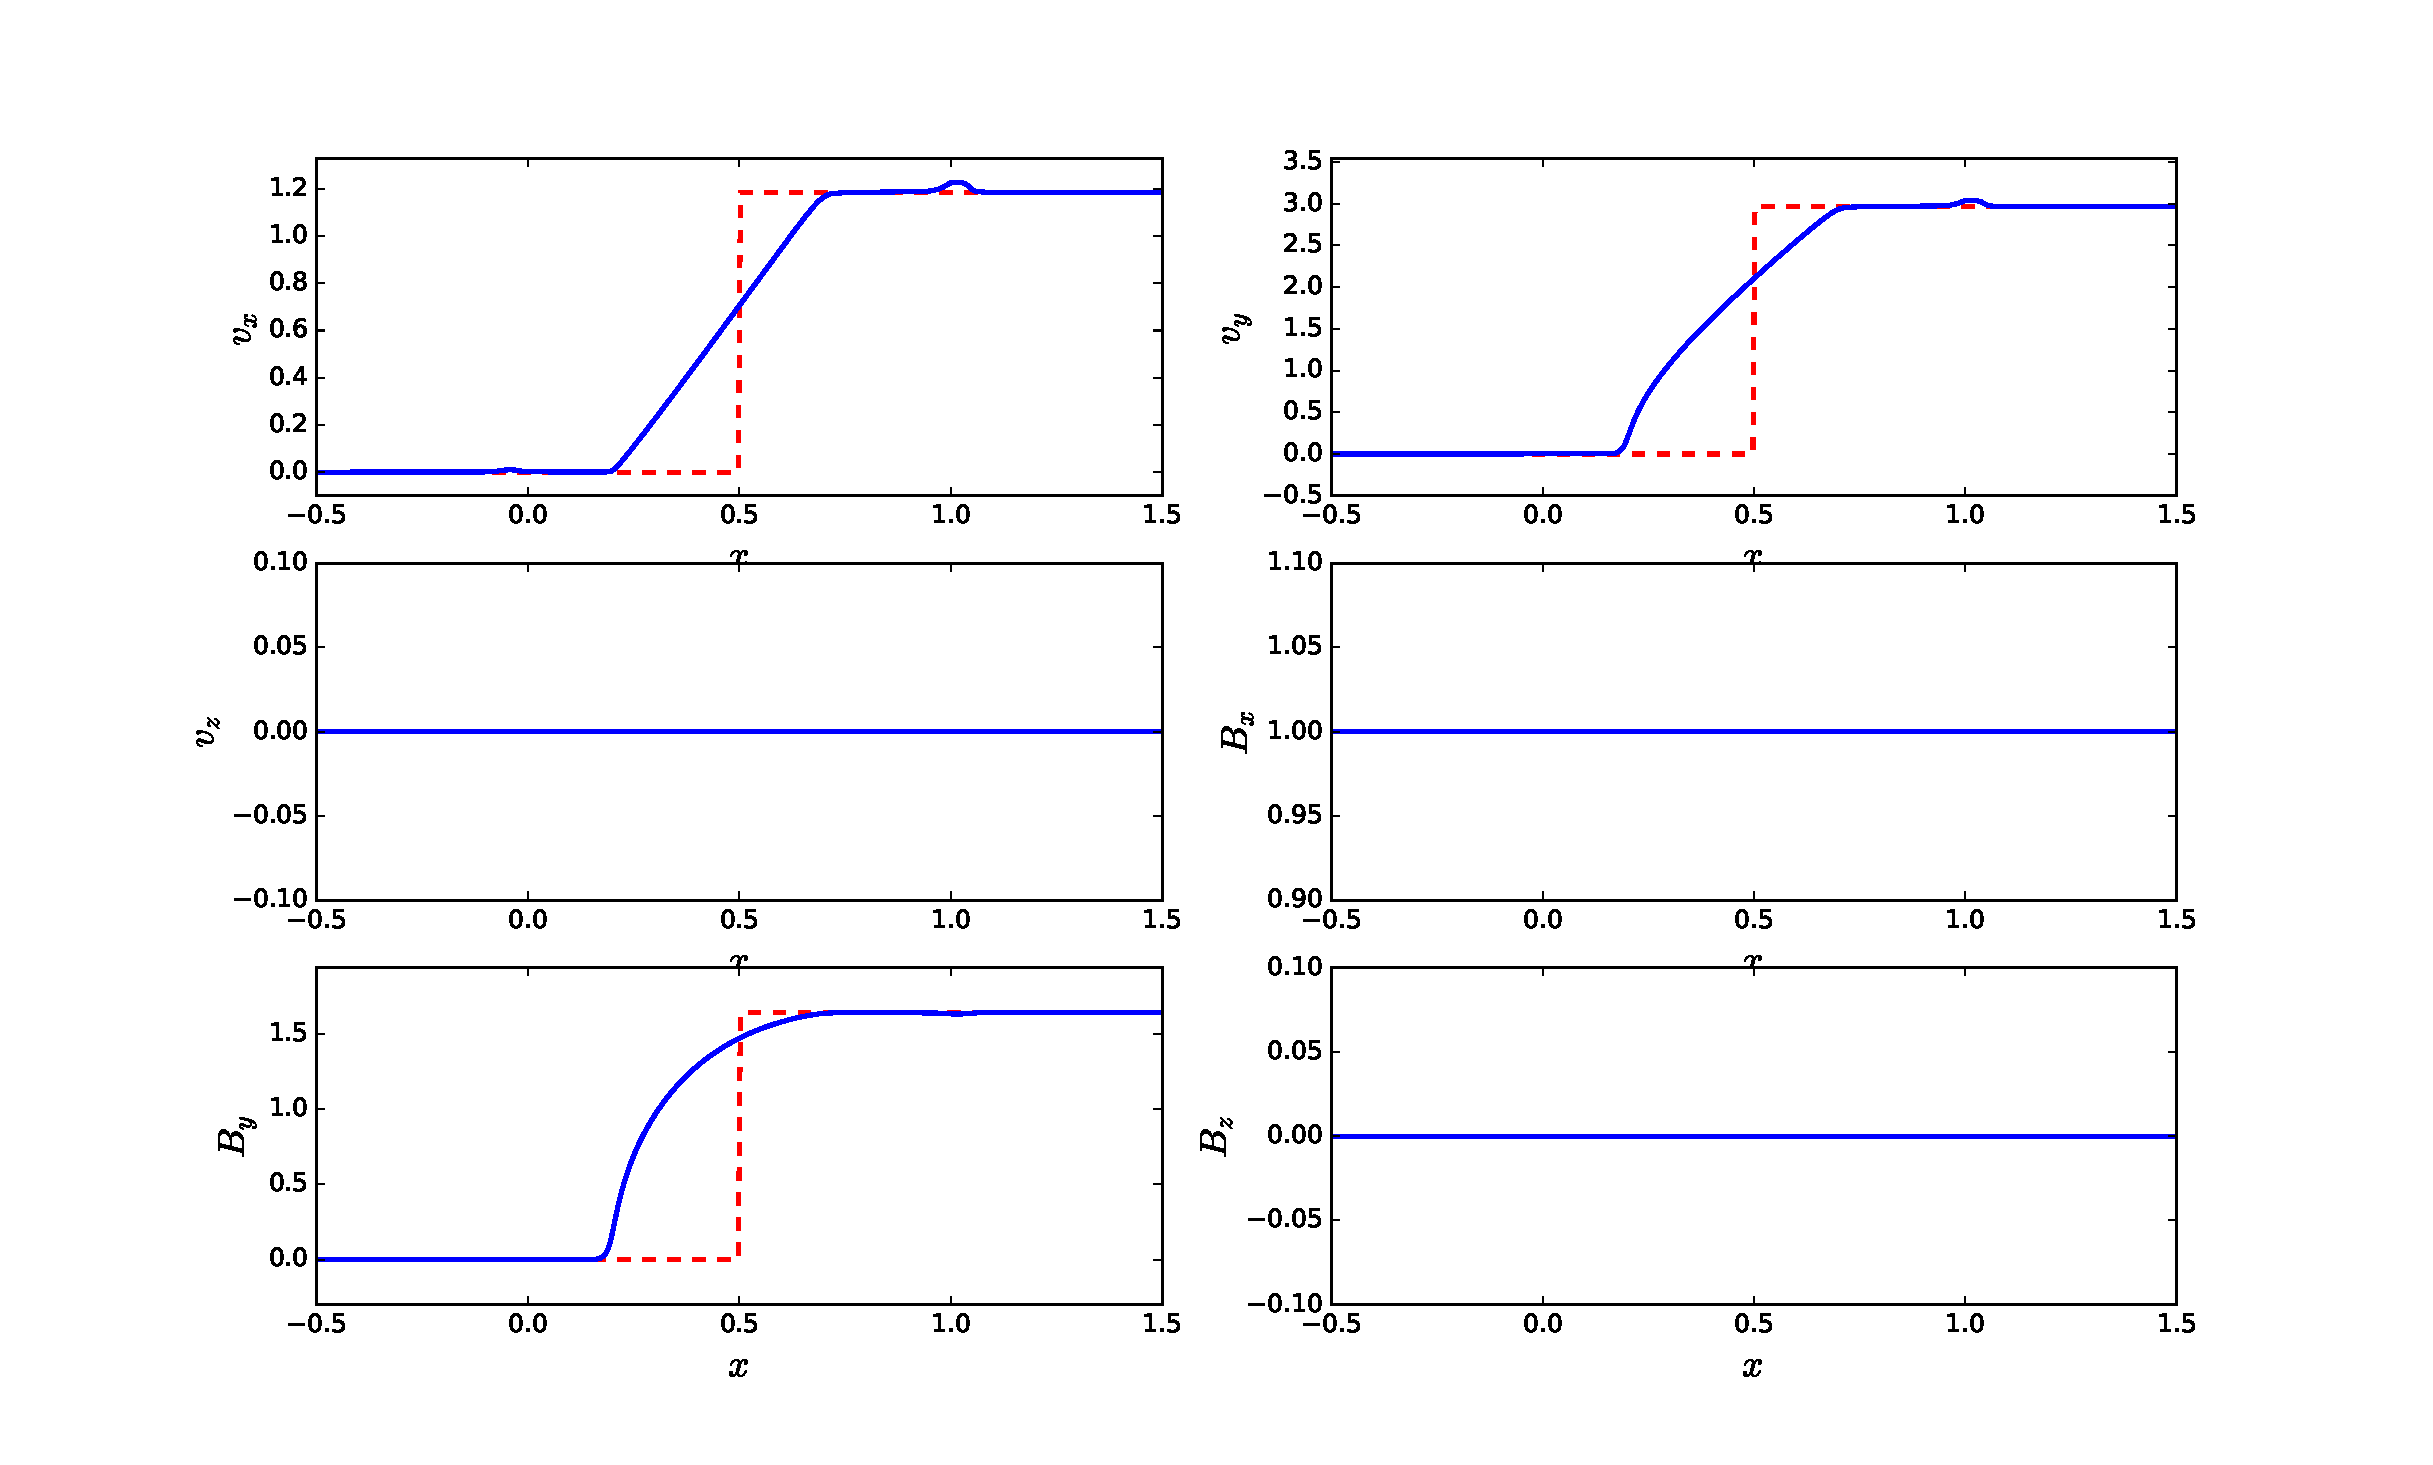
\includegraphics[width=1\textwidth]{SR2.eps}
	\end{minipage}%
\end{figure}
}
\tiny{$t_{\text{final}} =0.3$}
\end{frame}



\end{document}